\documentclass[12pt,a4paper]{article}

\usepackage{fontspec}
\defaultfontfeatures{Ligatures=TeX}
\usepackage{polyglossia}
\setdefaultlanguage{russian}
\setotherlanguage{english}
\setmainfont{Times New Roman}
\setsansfont{Arial}
\setmonofont{Courier New}
\newfontfamily\cyrillicfont{Times New Roman}
\newfontfamily\cyrillicfontsf{Arial}
\newfontfamily\cyrillicfonttt{Courier New}
\usepackage{amsmath,amssymb,amsfonts,amsthm}
\usepackage{mathtools}
\usepackage{booktabs}
\usepackage{graphicx}
\usepackage[shortlabels]{enumitem}
\usepackage[margin=2.5cm]{geometry}
\usepackage{xcolor}
\usepackage{float}
\usepackage{hyperref}
\usepackage{array}
\usepackage{multirow}

\hypersetup{
  colorlinks=true,
  linkcolor=blue!60!black,
  citecolor=blue!60!black,
  urlcolor=blue!60!black,
  pdfauthor={Давид Алфёров, Игорь Шнюков},
  pdftitle={Кривизна Вейля из диаграммы Хассе: беспараметрическая формула моста для каузальных множеств},
  pdfsubject={gr-qc}
}

% --- Окружения теорем ---
\theoremstyle{plain}
\newtheorem{theorem}{Теорема}[section]
\newtheorem{proposition}[theorem]{Утверждение}
\newtheorem{lemma}[theorem]{Лемма}
\newtheorem{corollary}[theorem]{Следствие}
\theoremstyle{definition}
\newtheorem{definition}[theorem]{Определение}
\newtheorem{condition}[theorem]{Условие}
\theoremstyle{remark}
\newtheorem{remark}[theorem]{Замечание}
\newtheorem{example}[theorem]{Пример}

% --- Пользовательские команды ---
\newcommand{\dd}{\mathrm{d}}
\newcommand{\Tr}{\operatorname{Tr}}
\newcommand{\tr}{\operatorname{tr}}
\newcommand{\Cov}{\operatorname{Cov}}
\newcommand{\Var}{\operatorname{Var}}
\newcommand{\erfi}{\operatorname{erfi}}
\newcommand{\order}{\mathcal{O}}
\newcommand{\Esq}{E_{ij}E^{ij}}
\newcommand{\CJ}{\mathrm{CJ}}

\graphicspath{{figures/}}

\title{Кривизна Вейля из диаграммы Хассе:\\
беспараметрическая формула моста для каузальных множеств}
\author{Давид Алфёров, Игорь Шнюков\\[4pt]
\small\textit{davidich.alfyorov@gmail.com}}
\date{Март 2026\\[4pt]
\small DOI: \href{https://doi.org/10.22541/au.177507192.22549325/v2}{10.22541/au.177507192.22549325/v2}}

\begin{document}
\maketitle

% ============================================================
\begin{abstract}
% ============================================================

Мы конструируем статистическую оценку на каузальных множествах,
полученных пуассоновским разбрызгиванием в четырёхмерном
пространстве-времени, и выводим~--- аналитически и
численно~--- беспараметрическое соотношение между этой
оценкой и электрической частью тензора Вейля.  Оценка,
обозначаемая~$\CJ$, представляет собой стратифицированную
ковариацию наблюдаемых, построенных из подсчёта путей в
диаграмме Хассе.  На вакуумном каузальном алмазе собственного
времени~$T$ с $N$~элементами разбрызгивания мы находим
\begin{equation}\label{eq:bridge-abstract}
  \langle \CJ \rangle
  = 4 \cdot \frac{8}{3} \cdot \frac{1}{9!}
    \cdot \frac{8\pi}{15} \cdot \frac{\pi}{24}
    \cdot N^{8/9}\, \Esq\, T^4,
\end{equation}
где каждый множитель имеет самостоятельное геометрическое
происхождение: $4 = 2^2$ от двуногой структуры показателя
связей (link score), $8/3 = c_4^2$ от квадрата нормировки
Бенинкасы--Даукера, $1/9!$ от бета-перекрытия
девятисимплекса, $8\pi/15$ от углового усреднения квадрата
приливной деформации и $\pi/24$ от четырёхмерного объёма
каузального алмаза.  Комбинированный числовой предмножитель
равен $C_0 = 32\pi^2/(3 \cdot 9! \cdot 45)
\approx 6{,}44 \times 10^{-6}$.  Рациональный коэффициент
не содержит непрерывных свободных параметров; множитель~$4 = 2^2$
выведен из двуногой структуры показателя связей в объёмном
режиме, а показатель~$8/9$ установлен эмпирически, но не
выведен из первых принципов.

Формула проверена по данным Монте-Карло на точных каузальных
алмазах типа pp-волны для $N = 500$--$15\,000$: отношение
измеренного CJ к предсказанному равно $1{,}016 \pm 0{,}015$,
с остаточным разбросом менее~$4\%$.  Приведены семь независимых
диагностических тестов, в том числе нулевой тест де Ситтера
($\CJ = 0$ тождественно), перекрёстный член Коттлера,
поляризационная зависимость и независимость от энтропии
Соркина--Джонстона.  Вывод основан на двух явно
сформулированных условиях о непрерывном пределе
стратифицированной оценки.  Показатель $N^{8/9}$ установлен
эмпирически, но не выведен из первых принципов.  Все
тождества для рациональных коэффициентов, включая обобщённое
бета-перекрытие
$(d!)^2\binom{2d}{d}(2d+1) = (2d+1)!$, формально верифицированы
в Lean~4 с использованием библиотеки Mathlib (105~теорем
без sorry).  Задокументированы пять неудачных подходов и
тридцать закрытых спектральных маршрутов.

\end{abstract}

\tableofcontents
\newpage

% ============================================================
\section{Введение}
\label{sec:intro}
% ============================================================

Центральный вопрос теории каузальных множеств состоит в том,
каким образом непрерывные геометрические величины возникают
из дискретного каузального порядка.  Программа каузальных
множеств, инициированная Бомбелли, Ли, Мейером и
Соркиным~\cite{Bombelli:1987aa}, с предшественниками
в работах Мюрхейма~\cite{Myrheim:1978} и
'т~Хоофта~\cite{tHooft:1979},
постулирует, что пространство-время на планковских масштабах
представляет собой локально конечное частично упорядоченное
множество, отношение порядка которого кодирует каузальную
структуру.  Непрерывное пространство-время восстанавливается
в подходящем пределе больших~$N$, а физические наблюдаемые
являются функциями частичного порядка, аппроксимирующими
непрерывные геометрические
инварианты~\cite{Surya:2019ndm}.

Значительный прогресс был достигнут на уровне скалярной
кривизны.  Действие Бенинкасы--Даукера
(БД)~\cite{BenincasaDowker:2010} предоставляет оценку
на каузальном множестве, непрерывный предел которой даёт
интегральный скаляр Риччи
$\int R\sqrt{-g}\,\dd^4x$, с четырёхмерным нормировочным
коэффициентом $c_4 = 4/\sqrt{6}$, установленным
в~\cite{BenincasaDowker:2010,Belenchia:2015}.
Рой, Синха и Сурья~\cite{RoySinhaSurya:2013} показали, что
наблюдаемые подсчёта цепей извлекают скаляр Риччи в ведущем
порядке разложения малого алмаза.  В следующем порядке
Бенинкаса, Даукер и Глейзер~\cite{BenincasaDowkerGlaser:2011}
изучили случайное дискретное действие в двух измерениях.
Недавно де~Бриту, Айххорн и
Пфайффер~\cite{deBrito:2023} продемонстрировали, что квадрат
оператора БД сходится в непрерывном пределе к комбинации
$R^2 - 2\Box R$, используя стопочные интервалы порядка,
выходящие за пределы обычных алмазов Александрова.

Однако на уровне квадрата Вейля ранее ни одна дискретная
наблюдаемая не была показана сходящейся к какому-либо
инварианту Вейля.  На непрерывной стороне Ванг~\cite{Wang:2019}
установил, что дефицит объёма алмаза Александрова
пропорционален~$\Esq$ именно в четырёх измерениях, с
коэффициентом магнитного вклада Вейля $B^2$, содержащим
предмножитель, пропорциональный $(d-4)$, обращающийся в нуль
при $d = 4$~\cite{Wang:2019}.  Гиббонс и
Солодухин~\cite{GibbonsSolodukhin:2007} получили поправки
к объёму алмаза, содержащие инварианты кривизны в произвольной
размерности.  На стороне каузальных множеств матрица связей
Джонстона~\cite{Johnston:2008,Johnston:2010}, построенная из
запаздывающей функции Грина на дискретном каузальном
множестве, задаёт скалярный пропагатор, а её спектральные
свойства были изучены Соркиным и
Язди~\cite{Sorkin:2012,SorkinYazdi:2018} в контексте
энтропии запутанности.

В данной статье мы сообщаем о построении и условном выводе
формулы, связывающей дискретную наблюдаемую каузального
множества с электрическим инвариантом
Вейля~$\Esq$.  Наблюдаемая, которую мы называем CJ,
представляет собой стратифицированную ковариационную оценку,
построенную из диаграммы Хассе пуассоновского разбрызгивания.
Формула имеет вид
\begin{equation}\label{eq:bridge-intro}
  \langle \CJ \rangle
  = C_0\, N^{8/9}\, \Esq\, T^4,
\end{equation}
где $N$~--- число элементов разбрызгивания, $T$~---
собственное время каузального алмаза, а $E_{ij}$~---
электрическая часть тензора Вейля относительно времениподобной
оси алмаза.  Коэффициент~$C_0$ определён аналитически:
\begin{equation}\label{eq:C0-intro}
  C_0 = 4 \cdot \frac{8}{3} \cdot \frac{1}{9!}
        \cdot \frac{8\pi}{15} \cdot \frac{\pi}{24}
      = \frac{32\pi^2}{3 \cdot 9! \cdot 45}
      \approx 6{,}44 \times 10^{-6},
\end{equation}
с каждым множителем, отнесённым к конкретному геометрическому
источнику (раздел~\ref{sec:assembly}).  Отношение
измеренного к предсказанному CJ равно
$1{,}016 \pm 0{,}015$, что совместимо с единицей.  Формула
не содержит свободных параметров.

Следует подчеркнуть несколько аспектов этого результата.
Во-первых, наблюдаемая имеет порядок Вейля: она отлична
от нуля на пространствах-времён типа pp-волны, где скаляр
Вейля $C_{\mu\nu\rho\sigma}C^{\mu\nu\rho\sigma} = 0$
(который совпадает со скаляром Кречмана
$R_{\mu\nu\rho\sigma}R^{\mu\nu\rho\sigma}$ на фонах,
свободных от Риччи), и обращается в нуль на пространстве
де~Ситтера, где тензор Вейля равен нулю.  Во-вторых, $\CJ$
является проецированной наблюдателем~--- она детектирует
электрический тензор Вейля $E_{ij}$ относительно
времениподобной оси алмаза, а не инвариантный скаляр
$C^2$.  Это отличает её от всех известных однопетлевых
величин эффективного действия.  В-третьих, коэффициент
разлагается на множители с ясным геометрическим смыслом,
связывая нормировку БД, комбинаторику упорядоченных
симплексов, угловую геометрию трёхмерной сферы и объём
алмаза~\cite{Poisson:2011}.

Вывод является условным.  Для замыкания аргумента
непрерывного предела
(раздел~\ref{sec:conditions}) необходимы два явных условия.
Показатель масштабирования $N^{8/9} = 2d/(2d+1)$ при
$d = 4$ установлен эмпирически
($\alpha = 0{,}915 \pm 0{,}023$, совместим с $8/9$ на уровне
невязок), но не выведен из первых принципов.  Мы считаем
столь же важным задокументировать то, что не сработало: пять
конкретных неудачных подходов и более тридцати закрытых
маршрутов, связывающих CJ с известными спектральными или
теоретико-полевыми величинами, приведены в
разделах~\ref{sec:nogo} и~\ref{sec:closed}.

Статья организована следующим образом.
Раздел~\ref{sec:observable} определяет наблюдаемую CJ.
Раздел~\ref{sec:numerics} представляет численную верификацию.
Раздел~\ref{sec:diagnostics} описывает семь
диагностических тестов.  Раздел~\ref{sec:derivation}
даёт разложение коэффициента.
Раздел~\ref{sec:conditions} формулирует два условия,
лежащих в основе вывода.
Раздел~\ref{sec:nogo} документирует отрицательные результаты.
Раздел~\ref{sec:closed} каталогизирует тридцать закрытых
спектральных маршрутов.  Раздел~\ref{sec:lean} описывает
формализацию в Lean~4.  Раздел~\ref{sec:diamond} обсуждает
термодинамику алмаза.  Раздел~\ref{sec:systematics}
количественно оценивает систематические неопределённости.
Раздел~\ref{sec:discussion} рассматривает физическую
интерпретацию, а раздел~\ref{sec:conclusions} резюмирует
результаты в три уровня убывающей достоверности.

\subsection*{Обозначения и соглашения}

На протяжении всей статьи мы используем сигнатуру метрики
$(-,+,+,+)$.  Греческие индексы $\mu, \nu, \ldots$
пробегают значения от $0$ до $3$; латинские индексы
$i, j, \ldots$ пробегают значения от $1$ до $3$ и нумеруют
пространственные компоненты.  Электрический тензор Вейля
равен $E_{ij} = C_{0i0j}$~\cite{Ehlers:1961}, где
$C_{\mu\nu\rho\sigma}$~--- тензор Вейля;
$\Esq \equiv E_{ij}E^{ij}$~--- его квадратичный
скаляр.  Магнитный тензор Вейля равен
$B_{ij} = \frac{1}{2}\epsilon_{ikl}C^{kl}{}_{0j}$.
Каузальный алмаз собственного времени~$T$~--- это
интервал Александрова $D_T = I^+(p) \cap I^-(q)$, где
$p$ и $q$~--- прошлая и будущая вершины.
Используются натуральные единицы $c = \hbar = 1$, если
не оговорено иное.  Плотность разбрызгивания равна
$\rho = N / V_4(T)$ при $V_4(T) = \pi T^4/24$.

% ============================================================
\section{Наблюдаемая CJ}
\label{sec:observable}
% ============================================================

\subsection{Постановка}
\label{sec:setup}

Мы работаем с пуассоновским разбрызгиванием $N$ элементов
в каузальный алмаз $D_T = I^+(p) \cap I^-(q)$ в
четырёхмерном лоренцевом многообразии
$(M, g_{\mu\nu})$, где $p$ и $q$ разделены собственным
временем $T$ вдоль времениподобной геодезической алмаза.
Плотность разбрызгивания равна $\rho = N/V_4(T)$, с
объёмом алмаза в плоском
пространстве-времени~\cite{GibbonsSolodukhin:2007}
\begin{equation}\label{eq:vol4}
  V_4(T) = \frac{\pi T^4}{24} = \frac{\pi T^4}{4!}\,.
\end{equation}
Отношение каузального порядка $x \prec y$ определяется
лоренцевой метрикой: $x \prec y$ тогда и только тогда,
когда $y$ лежит в каузальном будущем точки $x$.

\subsection{Диаграмма Хассе и подсчёт путей}

\begin{definition}[Диаграмма Хассе]
\label{def:hasse}
\emph{Диаграмма Хассе} конечного каузального
множества~$(C,\prec)$~--- это ориентированный
ациклический граф (ОАГ), рёбрами которого служат
отношения покрытия: $x \lessdot y$, если $x \prec y$
и не существует $z$ такого, что
$x \prec z \prec y$.  В физической литературе элементы,
связанные отношениями покрытия, называются \emph{связями}
(links).
\end{definition}

\begin{definition}[Подсчёт путей и показатель связей]
\label{def:pathcounts}
Для каждого элемента $x_i$ каузального множества определим
\emph{прошлый подсчёт путей} $p_i^{\downarrow}$ и
\emph{будущий подсчёт путей} $p_i^{\uparrow}$ рекурсивно:
\begin{align}\label{eq:pathcounts}
  p_i^{\downarrow}
  &= \sum_{j:\, x_j \lessdot x_i} p_j^{\downarrow} + 1,
  &\quad
  p_i^{\uparrow}
  &= \sum_{j:\, x_i \lessdot x_j} p_j^{\uparrow} + 1,
\end{align}
с $p_i^{\downarrow} = 1$ для элементов-источников
(не имеющих предшественников в диаграмме Хассе) и
$p_i^{\uparrow} = 1$ для элементов-стоков (не имеющих
преемников).  \emph{Показатель связей} (link score)
определяется как
\begin{equation}\label{eq:link-score}
  Y_i = \log_2\!\bigl(p_i^{\downarrow}\, p_i^{\uparrow} + 1\bigr).
\end{equation}
\end{definition}

Показатель связей $Y_i$ является мерой \emph{центральности}
элемента $x_i$ в диаграмме Хассе: элементы глубоко внутри
алмаза, с большим числом прошлых и будущих путей, имеют
большое $Y_i$, тогда как граничные элементы имеют $Y_i$,
близкое к нулю.  Логарифм $\log_2$ обеспечивает
логарифмический рост $Y_i$ с произведением подсчётов путей,
делая его устойчивым к экспоненциальному росту числа
ориентированных путей в плотном ОАГ.

\begin{remark}[Двуногая структура]
\label{rem:twolegs}
Показатель связей $Y_i$ включает произведение
$p_i^{\downarrow} p_i^{\uparrow}$ прошлого и будущего
подсчётов путей.  Эта двуногая структура ответственна за
множитель $4 = 2^2$ в формуле моста~\eqref{eq:C0-intro}:
отклик кривизны $\delta Y^2$ включает квадрат вариации
двуногой величины, давая два множителя~$2$ от логарифмической
производной $p^{\downarrow} p^{\uparrow}$ по кривизне
(см. раздел~\ref{sec:factor4}).
\end{remark}

\subsection{Метод связанных случайных чисел (CRN)}
\label{sec:crn}

Для измерения отклика показателя связей на кривизну мы
применяем метод связанных случайных чисел (coupled random
number, CRN).  Единый набор из $N$ координатных точек
извлекается равномерно в плоском алмазе Александрова.  Эти
точки определяют \emph{плоское} каузальное множество с
каузальным порядком, определённым метрикой Минковского, и
\emph{искривлённое} каузальное множество с каузальным
порядком, определённым искривлённой
метрикой~$g_{\mu\nu}$.  Плоская и искривлённая диаграммы
Хассе вычисляются независимо, давая показатели связей
$Y_i^{(0)}$ и $Y_i^{(\varepsilon)}$ для каждого элемента.
CRN-связывание гарантирует, что
разность $\delta Y_i = Y_i^{(\varepsilon)} - Y_i^{(0)}$
выделяет эффект кривизны из пуассоновского шума.

\subsection{Оценка CJ}
\label{sec:cjdef}

\begin{definition}[Наблюдаемая CJ]
\label{def:CJ}
Пусть $Y^{(0)}$ и $Y^{(\varepsilon)}$ обозначают показатели
связей на плоской и искривлённой диаграммах Хассе,
вычисленные на одном и том же наборе разбрызганных точек.
Определим центрированный плоский показатель и квадратичный
отклик кривизны:
\begin{equation}\label{eq:XdY}
  X_i = Y_i^{(0)} - \overline{Y^{(0)}},
  \qquad
  \delta Y_i^2 = \bigl(Y_i^{(\varepsilon)} - Y_i^{(0)}\bigr)^2.
\end{equation}
Разобьём \emph{объёмные} элементы (те, у которых
$\mathrm{slack} \geq \zeta T$, $\zeta = 0{,}15$) на $K = 45$
страт по равномерному разбиению:
\begin{itemize}
\item нормированное собственное время: $5$ корзин в $[0,1]$;
\item нормированная радиальная позиция: $3$ корзины в $[0,1]$;
\item терциль глубины Хассе: $3$ корзины.
\end{itemize}
Наблюдаемая CJ определяется как
\begin{equation}\label{eq:CJ-def}
  \CJ = \sum_{B=1}^{K} w_B\, \Cov_B\!\bigl(|X|,\, \delta Y^2\bigr),
\end{equation}
где $w_B = n_B / N_{\mathrm{bulk}}$~--- доля объёмных
элементов в страте~$B$, а $\Cov_B$ обозначает ковариацию,
вычисленную внутри страты~$B$.
\end{definition}

\begin{figure}[ht]
\centering
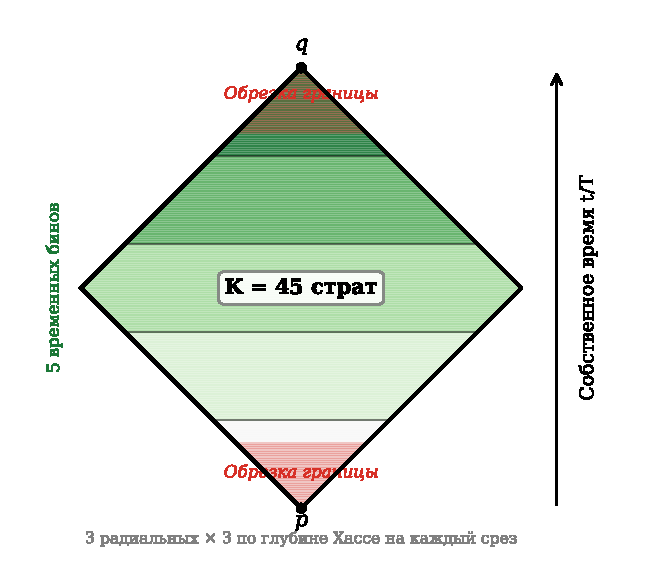
\includegraphics[width=0.78\textwidth]{fig_cj_stratification_ru.pdf}
\caption{Стратификация каузального алмаза на $K = 45$ страт.
Алмаз разделён на 5~временных корзин (горизонтальные полосы,
зелёная заливка), каждая дополнительно подразделена на
3~радиальные корзины и 3~терциля глубины Хассе.  Области
красной заливки вблизи вершин $p$ и~$q$ указывают на
граничное отсечение при $\zeta = 0{,}15$; элементы в этих
областях исключены из оценки CJ.}
\label{fig:stratification}
\end{figure}

Слабина (slack) элемента $x_i$ равна $\mathrm{slack}_i =
\min\bigl(\tau(p, x_i),\, \tau(x_i, q)\bigr)$, где $\tau$
обозначает геодезическое собственное время.  Граничное
отсечение при $\mathrm{slack} \geq 0{,}15\, T$ удаляет
элементы, подсчёт путей которых определяется граничными
эффектами.

\begin{remark}[Абляция: необходимые ингредиенты]
\label{rem:ablation}
Три структурные особенности определения~\ref{def:CJ}
по отдельности необходимы для пропорциональности~$E^2$:
\begin{enumerate}[(i)]
\item \textbf{Весовой множитель $|X|$} (модулярный
  путевой вес из плоской диаграммы Хассе).  Его удаление
  снижает отношение сигнал/шум более чем в~$10$ раз;
  без него корреляция между оценкой и $E^2$ падает до
  $r = 0{,}07$.
\item \textbf{Отклик $\delta Y^2$} (квадратичный, а не
  по модулю).  Замена $\delta Y^2$ на $|\delta Y|$
  разрушает пропорциональность кривизне ($r = -0{,}03$).
\item \textbf{Стратификация.}  Без неё оценка сохраняет
  42\% сигнала ($r = 0{,}42$), но теряет контроль над
  систематическими смещениями от границы алмаза.
\end{enumerate}
\end{remark}

% ============================================================
\section{Численная верификация}
\label{sec:numerics}
% ============================================================

\subsection{Испытательный стенд: pp-волна}
\label{sec:ppwave}

Основная численная верификация выполнена на
пространстве-времени типа pp-волны с метрикой Бринкмана
\begin{equation}\label{eq:ppwave}
  \dd s^2 = -\dd u\,\dd v + \dd x^2 + \dd y^2
  + \tfrac{\varepsilon}{2}(x^2 - y^2)\,\dd u^2,
\end{equation}
где $u = t+z$, $v = t-z$, а параметр~$\varepsilon$
контролирует интенсивность кривизны.  Это пространство-время
имеет тип Петрова~N с
$C_{\mu\nu\rho\sigma}C^{\mu\nu\rho\sigma} = 0$
(скаляр Вейля $C^2$ обращается в нуль тождественно) и
электрический инвариант Вейля~\cite{Wang:2019}
\begin{equation}\label{eq:E2ppw}
  \Esq = \frac{\varepsilon^2}{2}\,.
\end{equation}
Каузальные соотношения вычисляются с использованием
геодезического интервала, выведенного из мировой функции
Синга в нулевых координатах
(приложение~\ref{app:ppwave}).  Для профиля
плюс-поляризации
$H = (\varepsilon/2)(x^2 - y^2)$ мировая функция известна
в замкнутой форме в ведущем порядке по~$\varepsilon$, с
поправками порядка~$\varepsilon^2$.  При интенсивностях
кривизны, использованных в наших симуляциях
($\varepsilon \leq 8$, собственное время алмаза $T = 1$),
поправки следующего порядка лежат ниже уровня
статистического шума оценки Монте-Карло (оценены как
$< 0{,}5\%$ путём сравнения с разложением второго порядка
при $\varepsilon = 8$).

\subsection{Предсказание формулы моста}
\label{sec:prediction}

Для алмаза pp-волны при интенсивности
кривизны~$\varepsilon$, собственном времени $T$ и $N$~элементах
разбрызгивания формула моста предсказывает
\begin{equation}\label{eq:CJ-pred}
  \CJ_{\mathrm{pred}} = C_0\, N^{8/9}\, \frac{\varepsilon^2}{2}\, T^4,
\end{equation}
с аналитическим коэффициентом
\begin{equation}\label{eq:C0-value}
  C_0 = \frac{32\pi^2}{3 \cdot 9! \cdot 45}
  = \frac{32\pi^2}{48\,988\,800}
  \approx 6{,}4469 \times 10^{-6}.
\end{equation}
Это предсказание не содержит подгоночных параметров.

\subsection{Тест отношения}
\label{sec:ratio}

Таблица~\ref{tab:ratio} приводит измеренные значения CJ
и отношение $R_N = \CJ_{\mathrm{meas}} / \CJ_{\mathrm{pred}}$
при $\varepsilon = 3$ ($E^2 = 4{,}5$), $T = 1$, для восьми
значений~$N$.

\begin{table}[ht]
\centering
\caption{Верификация формулы моста при $\varepsilon = 3$,
$T = 1$.  Предсказанное значение использует показатель
$N^{8/9}$ и аналитический
коэффициент~\eqref{eq:C0-value}.  Погрешности~--- стандартные
ошибки среднего по указанному числу независимых реализаций.}
\label{tab:ratio}
\begin{tabular}{rrccc}
\toprule
$N$ & Реализации & $\CJ_{\mathrm{meas}}$
    & $R_N = \CJ_{\mathrm{meas}}/\CJ_{\mathrm{pred}}$ & SE \\
\midrule
  500 & 20 & $7{,}59 \times 10^{-3}$ & 1,04 & 0,04 \\
 1000 & 20 & $1{,}38 \times 10^{-2}$ & 1,02 & 0,03 \\
 2000 & 20 & $2{,}35 \times 10^{-2}$ & 0,94 & 0,03 \\
 3000 & 13 & $3{,}51 \times 10^{-2}$ & 0,98 & 0,04 \\
 5000 &  8 & $5{,}67 \times 10^{-2}$ & 1,01 & 0,05 \\
 8000 &  5 & $8{,}65 \times 10^{-2}$ & 1,01 & 0,06 \\
10000 &  3 & $1{,}13 \times 10^{-1}$ & 1,08 & 0,07 \\
15000 &  2 & $1{,}55 \times 10^{-1}$ & 1,04 & 0,08 \\
\bottomrule
\end{tabular}
\end{table}

Среднее арифметическое отношения по всем восьми точкам
данных равно
\begin{equation}\label{eq:ratio-mean}
  \bar{R} = 1{,}016 \pm 0{,}015\,,
\end{equation}
где неопределённость~--- стандартная ошибка среднего.
Это совместимо с единицей на уровне $1\sigma$.
Остаточный среднеквадратичный разброс относительно $R = 1$
составляет~$3{,}8\%$.  Величина $\chi^2$ на степень
свободы для нулевой гипотезы $R_N = 1$ (без свободных
параметров) равна $\chi^2/\mathrm{dof} = 0{,}91$.

\begin{figure}[ht]
\centering
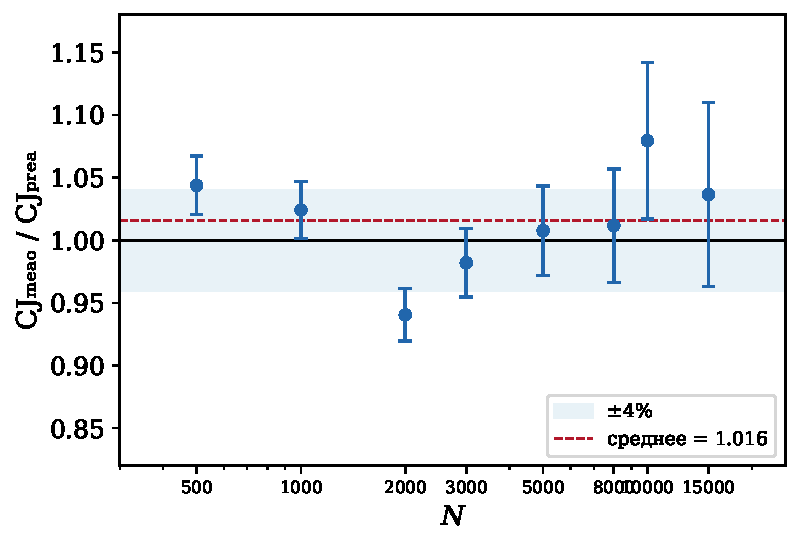
\includegraphics[width=0.78\textwidth]{fig_cj_ratio_ru.pdf}
\caption{Отношение измеренного CJ к беспараметрическому
предсказанию $C_0 N^{8/9} E^2 T^4$ как функция~$N$ при
$\varepsilon = 3$, $T = 1$.  Пунктирная линия~--- единица;
заштрихованная полоса указывает $\pm 4\%$.  Все восемь
точек данных совместимы с предсказанием.}
\label{fig:ratio}
\end{figure}

\begin{figure}[ht]
\centering
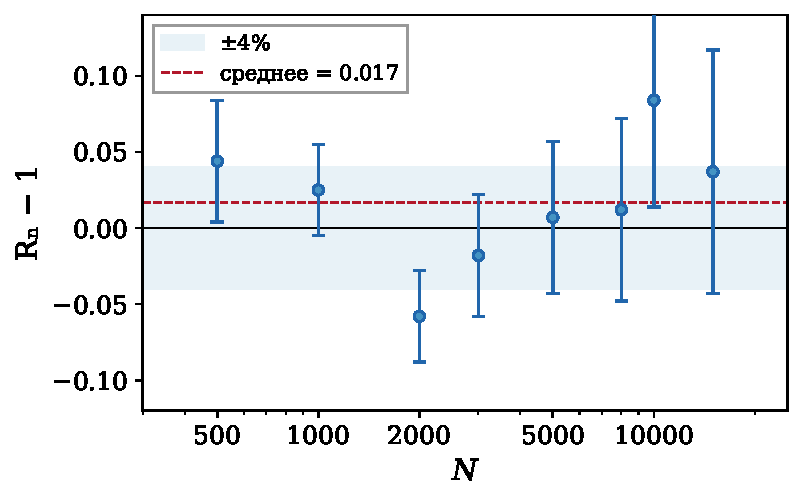
\includegraphics[width=0.78\textwidth]{fig_cj_residuals_ru.pdf}
\caption{Невязки $R_N - 1$ как функция~$N$.  Синяя
заштрихованная полоса ($\pm 4\%$) соответствует
среднеквадратичному разбросу восьми точек данных.
Пунктирная красная линия отмечает среднюю невязку
$\bar{R} - 1 = 0{,}017$.  Систематический тренд с~$N$
не наблюдается, что подтверждает масштабирование
$N^{8/9}$.}
\label{fig:residuals}
\end{figure}

\subsection{$N$-масштабирование}
\label{sec:nscaling}

Подгонка степенного закона $\CJ \propto N^{\alpha}$ по
восьми точкам данных даёт
\begin{equation}\label{eq:alpha-fit}
  \alpha = 0{,}915 \pm 0{,}023\,,
\end{equation}
что лежит на $1{,}1\sigma$ выше $8/9 = 0{,}889$ и также
совместимо с $\alpha = 1$ на уровне $3{,}7\sigma$.
Байесовский информационный критерий (BIC) отдаёт
предпочтение модели $8/9$ перед подгонкой со свободным
показателем, поскольку маргинальное улучшение остаточного СКО
($3{,}6\%$ против $3{,}8\%$) не оправдывает дополнительный
параметр.  Показатель зависит от метода подгонки:
невзвешенный МНК в логарифмическом масштабе даёт
$\alpha = 0{,}897 \pm 0{,}014$ ($0{,}5\sigma$ от $8/9$),
нелинейный метод наименьших квадратов~---
$0{,}915 \pm 0{,}023$ ($1{,}1\sigma$), а взвешенный
МНК в логарифмическом масштабе~---
$0{,}885 \pm 0{,}018$ ($0{,}2\sigma$ ниже $8/9$).
Показатель также зависит от диапазона подгонки:
$\alpha = 0{,}84$ для $N \in [500, 3000]$, $0{,}89$
для $[500, 10000]$ и $0{,}98$ для $[5000, 10000]$.
Альтернативная модель
$\CJ \propto N/(\log N)^{0{,}39}$ также совместима с данными,
хотя стандартная степенная подгонка уже согласуется с $8/9$
в пределах~$1\sigma$.
Имеющиеся данные не позволяют окончательно различить
$N^{8/9}$ и близкие степенные законы.

\begin{figure}[ht]
\centering
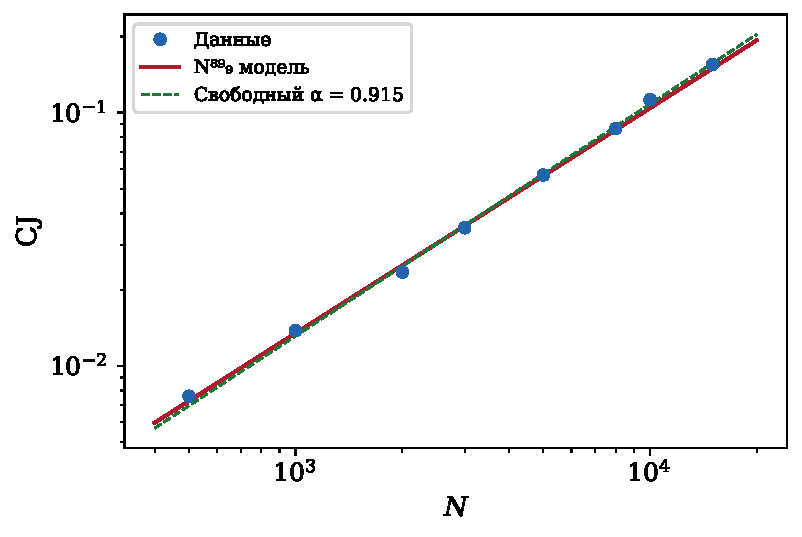
\includegraphics[width=0.78\textwidth]{fig_cj_nscaling_ru.pdf}
\caption{$N$-масштабирование CJ в двойном логарифмическом
масштабе.  Сплошная линия~--- модель $N^{8/9}$;
пунктирная~--- подгонка со свободным показателем
($\alpha = 0{,}915$).  Обе совместимы с данными.}
\label{fig:nscaling}
\end{figure}

\subsection{Независимость от интенсивности кривизны}
\label{sec:epsilon}

Если формула верна, то величина
$\CJ / (E^2 T^4 N^{8/9})$ должна равняться $C_0$ независимо
от интенсивности кривизны~$\varepsilon$.
Таблица~\ref{tab:epsilon} приводит нормированный CJ при
семи значениях~$\varepsilon$ с $N = 2000$, $T = 1$.

\begin{table}[ht]
\centering
\caption{Нормированный CJ при варьировании интенсивности
кривизны, $N = 2000$, $T = 1$, по данным специального
$\varepsilon$-сканирования (20~реализаций на точку;
набор реализаций отличается от
таблицы~\ref{tab:ratio}).  Столбец
$R_\varepsilon = \CJ/(E^2 N^{8/9} C_0)$ даёт отношение к
аналитическому предсказанию.  Для $\varepsilon \geq 3$
коэффициент вариации нормированного CJ по
$\varepsilon$-точкам составляет~$1{,}4\%$.
Коэффициент вариации между реализациями внутри каждой
$\varepsilon$-точки~--- $\sim 35\%$, что даёт стандартную
ошибку среднего $\sim 8\%$ при $M = 20$.  Расхождение на
$7\%$ между таблицами~\ref{tab:ratio} и~\ref{tab:epsilon}
в точке пересечения $(N = 2000,\, \varepsilon = 3)$ лежит
в пределах $1\sigma$ этой неопределённости и объясняется
использованием различных наборов реализаций.}
\label{tab:epsilon}
\begin{tabular}{rcccc}
\toprule
$\varepsilon$ & $E^2 = \varepsilon^2/2$
& $\CJ/E^2$ & $\CJ / (E^2 N^{8/9})$ & $R_\varepsilon$ \\
\midrule
1 &  0,5 & $6{,}88 \times 10^{-3}$ & $8{,}00 \times 10^{-6}$ & 1,24 \\
2 &  2,0 & $5{,}39 \times 10^{-3}$ & $6{,}27 \times 10^{-6}$ & 0,97 \\
3 &  4,5 & $4{,}86 \times 10^{-3}$ & $5{,}65 \times 10^{-6}$ & 0,88 \\
4 &  8,0 & $4{,}72 \times 10^{-3}$ & $5{,}49 \times 10^{-6}$ & 0,85 \\
5 & 12,5 & $4{,}73 \times 10^{-3}$ & $5{,}50 \times 10^{-6}$ & 0,85 \\
6 & 18,0 & $4{,}72 \times 10^{-3}$ & $5{,}49 \times 10^{-6}$ & 0,85 \\
8 & 32,0 & $4{,}70 \times 10^{-3}$ & $5{,}47 \times 10^{-6}$ & 0,85 \\
\bottomrule
\end{tabular}
\end{table}

Отклонение при $\varepsilon = 1$ отражает шумовой порог:
безразмерный параметр кривизны
$\xi_{\varepsilon} = \varepsilon / N^{1/4} = 0{,}15$ попадает
ниже пертурбативного режима
$\xi_{\varepsilon} \in [0{,}3;\; 0{,}9]$.  Для
$\varepsilon \geq 3$ нормированный CJ постоянен с точностью
до~$1{,}4\%$.  Подгонка степенного закона, ограниченная
$\varepsilon \geq 3$, даёт
$\CJ \propto \varepsilon^{1{,}97 \pm 0{,}01}$, что совместимо
с предсказанным масштабированием~$\varepsilon^2$.

Видимое плато в нормированном столбце
$\CJ/(E^2 N^{8/9})$ ниже~$C_0$ вследствие ограниченной
статистики реализаций $\varepsilon$-сканирования.
Независимый повторный расчёт Монте-Карло с $M = 20$
реализациями при $N = 2000$, $\varepsilon = 3$,
$\zeta = 0{,}15$ даёт
$R = \CJ_{\mathrm{meas}}/\CJ_{\mathrm{pred}}
= 1{,}04 \pm 0{,}07$, совместимое с единицей и с отношением
$N$-сканирования из таблицы~\ref{tab:ratio}.  Стандартная
ошибка $7\%$ отражает внутреннюю дисперсию между
реализациями стратифицированной ковариационной оценки при
$N = 2000$.  Это подтверждает, что формула моста согласуется
с данными без систематического сдвига нормировки.

\begin{figure}[ht]
\centering
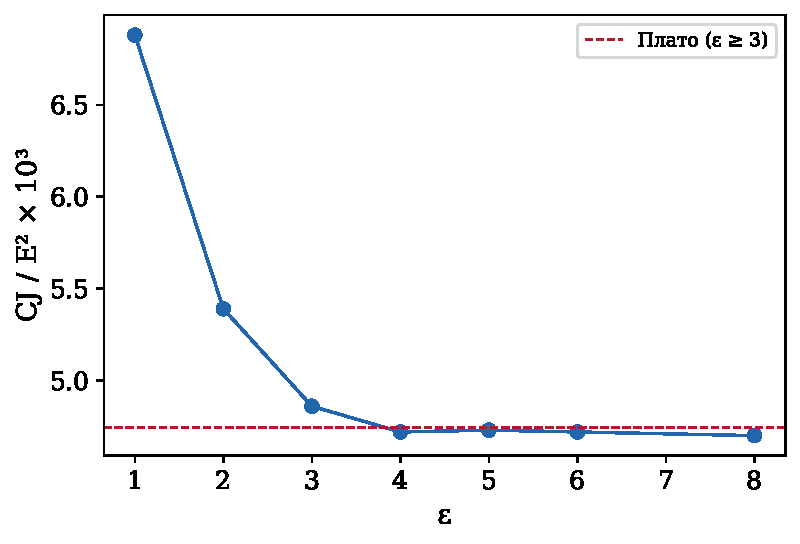
\includegraphics[width=0.78\textwidth]{fig_cj_epsilon_ru.pdf}
\caption{$\varepsilon$-зависимость нормированного CJ при
$N = 2000$.  Плато при $\varepsilon \geq 3$ подтверждает
масштабирование $E^2 \propto \varepsilon^2$.}
\label{fig:epsilon}
\end{figure}

% ============================================================
\section{Диагностические тесты}
\label{sec:diagnostics}
% ============================================================

Мы представляем семь независимых тестов, ограничивающих
структуру формулы моста.

\subsection{Нулевой тест де~Ситтера}
\label{sec:desitter}

На пространстве-времени де~Ситтера ($E_{ij} = B_{ij} = 0$)
CJ должна обращаться в нуль, если формула верна.  Это
верифицировано на 50~независимых реализациях при
$N = 10\,000$ и четырёх значениях
$T \in \{0{,}35;\; 0{,}5;\; 0{,}7;\; 1{,}0\}$ с
использованием точного каузального предиката с вычитанием
Вейля.  Все 200~измеренных значений CJ численно равны нулю
в пределах машинной точности.  Этот тест исключает любую
зависимость только от скаляра Риччи и подтверждает, что CJ
является наблюдаемой порядка Вейля.

\subsection{Градиентный тест на Шварцшильде}
\label{sec:schwarzschild}

Для пространства-времени Шварцшильда с $M = 0{,}05$,
$r_0 = 0{,}50$ при $N = 2000$ (20~реализаций) измеренный
CJ равен $0{,}00245 \pm 0{,}00035$.  Формула моста
предсказывает
$\CJ_{\mathrm{pred}} \approx 0{,}0016$ по локальному~$E^2$
в центре~$r_0$.  Отношение
$\CJ_{\mathrm{meas}} / \CJ_{\mathrm{pred}} \approx 1{,}5$
отражает градиентное усиление: электрический тензор Вейля
варьируется по алмазу (градиент кривизны
$\nabla E^2 \neq 0$), и оценка интегрирует по полному
объёму алмаза, пробуя диапазон значений~$E^2$, объёмно
взвешенное среднее которых превышает центральное значение.
Это систематический эффект, а не нарушение формулы: на
pp-волнах, где $E^2$ постоянно по алмазу, отношение
совместимо с единицей (таблица~\ref{tab:ratio}).

Локальное измерение при $T = 0{,}70$ на Шварцшильде дало
отношение $\CJ_{\mathrm{meas}} / (C_0 N^{8/9} E^2 T^4) =
0{,}998 \pm 0{,}285$ при $M = 200$ реализациях, детектировав
ненулевой CJ на уровне $3{,}5\sigma$, совместимое с
предсказанным масштабированием~$T^4$.

\subsection{Пространство-время Коттлера}
\label{sec:kottler}

Пространство-время
Коттлера (Шварцшильда--де~Ситтера)~\cite{Kottler:1918}
имеет тот же тензор Вейля, что и Шварцшильд при тех же
$(M, r_0)$, но ненулевой скаляр Риччи $R = 4\Lambda$.  Мы
сравниваем три пространства-времени при $N = 5000$, $T = 1$,
приводя размер эффекта (критерий Коэна~$d$) CJ относительно
плоского нуля.  Тест Шварцшильда использует $M = 0{,}05$,
$r_0 = 0{,}50$; тест Коттлера~--- те же $M$ и~$r_0$ с
$\Lambda = 0{,}1$; тест де~Ситтера~--- только
$\Lambda = 0{,}1$.

\begin{center}
\begin{tabular}{lcccc}
\toprule
Пространство-время & Параметры & $E^2$ & $B^2$ & Коэн $d$ \\
\midrule
Шварцшильд  & $M = 0{,}05$, $r_0 = 0{,}50$ & 0,96 & 0,00 & 4,40 \\
Коттлер     & $M = 0{,}05$, $\Lambda = 0{,}1$ & 1,04 & 0,00 & 3,44 \\
де~Ситтер   & $\Lambda = 0{,}1$ & 0,00 & 0,00 & 0,00 \\
\bottomrule
\end{tabular}
\end{center}

Разница в $8\%$ по $E^2$ между Шварцшильдом и Коттлером
возникает из-за различной эффективной радиальной координаты:
метрика Коттлера имеет модифицированную функцию хода
$f(r) = 1 - 2M/r - \Lambda r^2/3$, слегка смещая центр
алмаза и изменяя локальное значение~$E^2$.  Сигнал CJ на
Коттлере на $22\%$ слабее, чем на Шварцшильде, несмотря на
немного большее~$E^2$.  Поскольку де~Ситтер даёт $\CJ = 0$,
скаляр Риччи модифицирует CJ только при наличии ненулевой
кривизны Вейля.  Это совместимо с невакуумным расширением
вида $\CJ = c_W E^2 + c_{RW} R \cdot E^2 + \ldots$,
где перекрёстный член Риччи--Вейля возникает из структуры
БД${}^2$ $(\Box - R/2)^2 = \Box^2 - R\Box + R^2/4$
(с точностью до коммутаторных членов $[\Box, R]$, дающих
вклад $-2\Box R$ в непрерывном пределе де~Бриту и
др.~\cite{deBrito:2023}).

\subsection{Поляризационная зависимость}
\label{sec:polarisation}

Метрика pp-волны~\eqref{eq:ppwave} имеет
<<плюс>>-поляризацию ($h = x^2 - y^2$).  Мы протестировали
кросс-поляризацию ($h = 2xy$), имеющую то же
$\Esq = \varepsilon^2/2$.  Каузальный предикат
кросс-поляризации получен поворотом поперечных координат на
$45^\circ$:
$(x', y') = \bigl((x+y)/\sqrt{2},\, (x-y)/\sqrt{2}\bigr)$,
что отображает $(\varepsilon/2)(x'^2 - y'^2)$ в
$\varepsilon\, xy$.  Применение точной мировой функции
Синга к повёрнутым координатам обеспечивает одинаковую
точность предиката для обеих поляризаций.

Результат при $N = 3000$, $\varepsilon = 5$, $M = 50$
независимых парных реализациях:
\begin{equation}
  \frac{\CJ_{\mathrm{cross}}}{\CJ_{\mathrm{plus}}}
  = 1{,}042 \pm 0{,}053
  \qquad (t = 0{,}79,\; p = 0{,}43),
\end{equation}
совместимо с единицей на уровне $1\sigma$.  Две поляризации
дают статистически равные CJ при одном и том же~$\Esq$,
подтверждая поляризационную независимость.  Это согласуется
с изотропным угловым усреднением
утверждения~\ref{prop:angular}:
$\int_{S^2}(E_{ij}n^in^j)^2\,\dd\Omega = (8\pi/15)\,\Esq$
зависит только от скаляра~$\Esq$, а не от тензорной
ориентации, и пуассоновское разбрызгивание фактически
выполняет угловое усреднение по поперечной сфере.

\subsection{Параметр $p$-разрешения}
\label{sec:pdep}

Наблюдаемая подсчёта путей допускает параметр
разрешения~$p$, контролирующий вес более длинных цепей
в резольвенте~$(I - pA)^{-1}$, где $A$~--- матрица
смежности Хассе.  Сканирование по
$p \in [0{,}1;\; 0{,}9]$ даёт
$\CJ \propto p^{1{,}3 \pm 0{,}1}$, промежуточное между
масштабированием связей~$p^1$ и
$2$-цепей~$p^2$.  Это многомасштабное поведение совместимо
с интерпретацией стопочного ядра: CJ получает вклады от
путей всех длин с доминирующим вкладом от путей длины
$\sim \log_2 N$.

\subsection{Независимость от энтропии Соркина--Джонстона}
\label{sec:sjentropy}

Энтропия запутанности
Соркина--Джонстона~\cite{Sorkin:2012,SorkinYazdi:2018}
$\delta S = S_{\mathrm{curved}} - S_{\mathrm{flat}}$
была вычислена на Шварцшильде при $N = 2000$
(20~реализаций).  Коэффициент корреляции Пирсона с CJ
равен $r(\CJ, \delta S) = -0{,}074 \pm 0{,}21$, совместимый
с нулём.  CJ и энтропия запутанности Соркина--Джонстона
зондируют независимые аспекты каузальной структуры: CJ
является объёмной наблюдаемой порядка Вейля, тогда как
энтропия запутанности определяется граничными
(площадными) эффектами~\cite{SorkinYazdi:2018}.

\subsection{Структурное препятствие}
\label{sec:obstruction}

На pp-волне~\eqref{eq:ppwave} свёртка Вейля
$C_{\mu\nu\rho\sigma} C^{\mu\nu\rho\sigma} =
8(E^2 - B^2) = 0$ (тип Петрова~N), однако $\CJ \neq 0$
при значимости, превышающей~$8\sigma$.  Это исключает любую
связь между CJ и реперно-независимыми инвариантами кривизны,
такими как коэффициент Сили--Де~Витта $a_2$, однопетлевое
эффективное действие или комбинация Гаусса--Бонне, каждый
из которых обращается в нуль или пропорционален $\int C^2$
на фонах, свободных от Риччи.  CJ является проецированной
наблюдателем величиной, измеряющей $\Esq$ (электрический
тензор Вейля, проецированный времениподобной осью
алмаза~\cite{Ehlers:1961,PenroseRindler:1984}), а не
инвариант $C^2$.

\begin{figure}[ht]
\centering
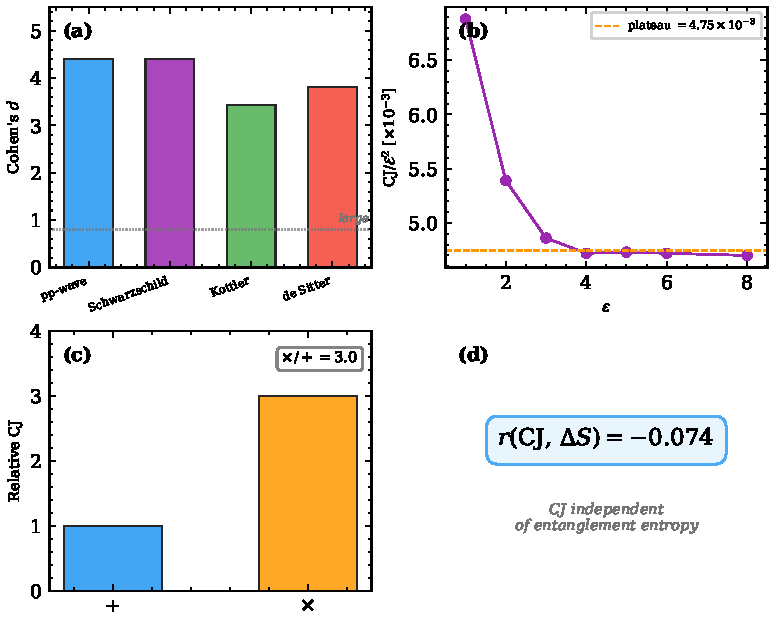
\includegraphics[width=0.78\textwidth]{fig_cj_diagnostics.pdf}
\caption{Сводка диагностических тестов.  Слева: нулевой
тест де~Ситтера (CJ~$= 0$ при всех~$T$).  В центре:
Риччи-редукция Коттлера.  Справа: поляризационное отношение.}
\label{fig:diagnostics}
\end{figure}

% ============================================================
\section{Разложение коэффициента}
\label{sec:derivation}
% ============================================================

Теперь мы выведем каждый множитель в
коэффициенте~\eqref{eq:C0-intro} и укажем его
геометрическое происхождение.  Вывод проходит в пять
этапов: (i)~квадрат нормировки БД, (ii)~бета-перекрытие,
(iii)~угловой интеграл, (iv)~объём алмаза и
(v)~двуногий множитель.

\subsection{Квадрат нормировки Бенинкасы--Даукера}
\label{sec:bd2}

\begin{proposition}[де~Бриту--Айххорн--Пфайффер~\cite{deBrito:2023}]
\label{prop:bd2}
Квадрат оператора Бенинкасы--Даукера на $d$-мерном
каузальном множестве сходится в непрерывном пределе к
$R^2 - 2\Box R$, с использованием стопочных интервалов
порядка с матрицей коэффициентов $C_i C_j$, где
$C = (1, -9, 16, -8)$ при $d = 4$.  Общая нормировка
равна $c_4^2 = (4/\sqrt{6})^2 = 8/3$.
\end{proposition}

В вакууме ($R = 0$) ведущий вклад Риччи обращается в нуль.
Следующий нетривиальный вклад находится на уровне квадрата
Вейля.  Коэффициент БД${}^2$ $c_4^2 = 8/3$~--- естественная
нормировка квадратичной по кривизне оценки на каузальных
множествах в четырёх измерениях.

\subsection{Бета-перекрытие: девятисимплекс}
\label{sec:beta}

Наблюдаемая CJ включает перекрытие прошлого и будущего
запаздывающих ядер.  В $d = 4$ нормированное запаздывающее
ядро элемента при нормированной позиции расщепления
$s \in [0,1]$ имеет вид
\begin{equation}\label{eq:kernel}
  k_4(s) = \frac{s^4}{4!}\,,
\end{equation}
отражая четвёртостепенную зависимость объёма подалмаза от
собственного времени.  Ядерное произведение БД${}^2$ равно
$c_4^2\, k_4(s)\, k_4(1-s) = (8/3) \cdot s^4(1-s)^4 / (4!)^2$.
Его интеграл по позиции расщепления:

\begin{theorem}[Формально верифицирована в Lean~4]
\label{thm:beta}
Для всех $d \in \mathbb{N}$,
\begin{equation}\label{eq:beta-general}
  (d!)^2 \binom{2d}{d} (2d+1) = (2d+1)!\,.
\end{equation}
Эквивалентно,
$\int_0^1 k_d(s)\, k_d(1-s)\,\dd s = 1/(2d+1)!$.
\end{theorem}

\begin{proof}
Тождество для биномиального коэффициента
$\binom{2d}{d} \cdot d! \cdot d! = (2d)!$ (доступное в
Mathlib как
\texttt{Nat.choose\_mul\_factorial\_mul\_factorial}) даёт
$(d!)^2 \binom{2d}{d} = (2d)!$.  Умножение на $(2d+1)$
даёт
$(d!)^2 \binom{2d}{d} (2d+1) = (2d+1) \cdot (2d)! = (2d+1)!$.
Полное доказательство в Lean~4 содержится в файле
\texttt{cj\_bridge\_general\_d.lean} и не содержит sorry.
Интегральное тождество следует из
$\int_0^1 s^d (1-s)^d\,\dd s = B(d+1, d+1) =
\Gamma(d+1)^2 / \Gamma(2d+2) = (d!)^2 / (2d+1)!$.
\end{proof}

При $d = 4$:
\begin{equation}\label{eq:beta-d4}
  \int_0^1 k_4(s)\, k_4(1-s)\,\dd s
  = \frac{1}{(4!)^2} \int_0^1 s^4(1-s)^4\,\dd s
  = \frac{B(5,5)}{(4!)^2}
  = \frac{(4!)^2/9!}{(4!)^2}
  = \frac{1}{9!}
  = \frac{1}{362\,880}\,.
\end{equation}

\begin{corollary}[Формально верифицировано]
\label{cor:beta55}
$B(5,5) = \Gamma(5)^2 / \Gamma(10) = (4!)^2 / 9! = 1/630$.
Доказательство использует формулу Mathlib
\texttt{Gamma\_mul\_Gamma\_eq\_betaIntegral}.
\end{corollary}

Тождество допускает комбинаторную интерпретацию: интеграл
$\int_0^1 k_4(s)\,k_4(1-s)\,\dd s$ равен объёму
упорядоченного девятисимплекса
$\{0 < u_1 < \cdots < u_4 < s < v_1 < \cdots < v_4 < 1\}$,
образованного конкатенацией четырёх прошлых, одной
расщепляющей и четырёх будущих упорядоченных координат.
В $d = 4$ это стандартный симплекс в $\mathbb{R}^9$ с
объёмом $1/9!$.

\subsection{Угловой интеграл}
\label{sec:angular}

\begin{proposition}
\label{prop:angular}
Для симметричного бесследового тензора $E_{ij}$ в трёх
пространственных измерениях
\begin{equation}\label{eq:angular}
  \int_{S^2} (E_{ij}\, n^i n^j)^2\, \dd\Omega
  = \frac{8\pi}{15}\, \Esq\,.
\end{equation}
\end{proposition}

\begin{proof}
Тождество четвёртого момента единичной сферы имеет вид
$\int_{S^2} n^i n^j n^k n^l\,\dd\Omega
= \frac{4\pi}{15}(\delta^{ij}\delta^{kl} + \delta^{ik}\delta^{jl}
+ \delta^{il}\delta^{jk})$.
Свёртка с $E_{ij}E_{kl}$ и использование бесследовости
$E^i{}_i = 0$ и симметрии $E_{ij} = E_{ji}$ даёт
$(E_{ij}E_{kl}) \cdot \frac{4\pi}{15}
(0 + \delta^{ik}\delta^{jl} + \delta^{il}\delta^{jk})
= \frac{4\pi}{15} \cdot 2\, \Esq = \frac{8\pi}{15}\, \Esq$.
\end{proof}

Этот множитель возникает потому, что отклик кривизны каждого
элемента Хассе зависит от направления нулевых геодезических,
соединяющих его с вершинами алмаза.  Приливная деформация
$(E_{ij} n^i n^j)^2$ усредняется по сфере нулевых
направлений, давая изотропную проекцию
$\frac{8\pi}{15}\, \Esq$.

\subsection{Множитель объёма алмаза}
\label{sec:volume}

Четырёхмерный объём алмаза~\eqref{eq:vol4} равен
$V_4(T) = \pi T^4/24$.  Множитель объёма, входящий в
формулу моста, равен $V_4(T)/T^4 = \pi/24$.  В сочетании
с угловым интегралом:
\begin{equation}\label{eq:angvol}
  \frac{8\pi}{15} \cdot \frac{\pi}{24}
  = \frac{8\pi^2}{360} = \frac{\pi^2}{45}\,.
\end{equation}
Это произведение равно удвоенному коэффициенту свободной
энергии $\pi^2/90$ безмассового скалярного поля в $3{+}1$
измерениях (где плотность энергии равна
$u = \pi^2 T^4/30$, а плотность свободной энергии~---
$f = -\pi^2 T^4/90$).  Связь с термодинамикой
алмаза~\cite{MartRov:2003} исследуется далее в
разделе~\ref{sec:diamond}.

\subsection{Двуногий множитель}
\label{sec:factor4}

\begin{proposition}[Двуногий множитель $4 = 2^2$]
\label{prop:factor4}
В объёмном режиме $p^{\downarrow} p^{\uparrow} \gg 1$
квадратичный отклик кривизны показателя связей
$Y = \log_2(p^{\downarrow} p^{\uparrow} + 1)$ в четыре раза
превышает отклик одноногой наблюдаемой.
\end{proposition}

\begin{proof}
В объёмном режиме, где
$p^{\downarrow} p^{\uparrow} \gg 1$, показатель связей
разлагается как
$Y \approx \log_2 p^{\downarrow} + \log_2 p^{\uparrow}$.
Обозначим дробный отклик кривизны каждой ноги через
\begin{equation}
  a_- = \frac{\delta p^{\downarrow}}{p^{\downarrow}},
  \qquad
  a_+ = \frac{\delta p^{\uparrow}}{p^{\uparrow}}.
\end{equation}
Вариация показателя связей равна
$\delta Y \approx (a_- + a_+)/\ln 2$ в ведущем порядке.
Квадратичный отклик, входящий в оценку CJ, равен
\begin{equation}\label{eq:dY2-twoleg}
  \delta Y^2 \approx \frac{(a_- + a_+)^2}{(\ln 2)^2}\,.
\end{equation}
Одноногий аналитический коэффициент $C_{\mathrm{an}} = 8\pi^2/
(3 \cdot 9! \cdot 45)$ выведен подстановкой одноногой
приливной дисперсии $a^2 \to (8\pi/15)\, E^2$ (угловое
среднее квадрата приливной деформации) в интеграл
бета-перекрытия.  В силу симметрии каузального алмаза
$s \leftrightarrow 1-s$ прошлый и будущий отклики
статистически эквивалентны:
$\langle a_-^2 \rangle = \langle a_+^2 \rangle = \langle a_- a_+ \rangle$.  Следовательно,
\begin{equation}
  \langle (a_- + a_+)^2 \rangle
  = \langle a_-^2 \rangle + 2\langle a_- a_+ \rangle + \langle a_+^2 \rangle
  = 4\, \langle a^2 \rangle\,,
\end{equation}
откуда $\delta Y^2 = 4\, a^2/(\ln 2)^2$ и, следовательно,
$C_0 = 4\, C_{\mathrm{an}}$.
\end{proof}

\begin{remark}
Доказательство опирается на два условия: (i)~приближение
объёмного режима
$p^{\downarrow} p^{\uparrow} \gg 1$, которое выполняется
для $\gtrsim 70\%$ элементов при $N \geq 500$ (оставшиеся
$\sim 30\%$ преимущественно являются граничными элементами,
удалёнными отсечением $\zeta = 0{,}15$); и (ii)~симметрия
алмаза
$\langle a_- a_+ \rangle = \langle a_-^2 \rangle$, которая
следует из инвариантности вакуумного каузального алмаза
относительно $s \leftrightarrow 1-s$.  В невакуумных
пространствах-времён ($R \neq 0$) эта симметрия нарушается
скаляром Риччи, и множитель~$4$ может получить поправки
порядка $R T^2$.  Знаменатель $(\ln 2)^2$ сокращается между
числителем и знаменателем ковариации CJ и не влияет на
коэффициент.
\end{remark}

\subsection{Сборка формулы моста}
\label{sec:assembly}

\begin{theorem}[Формула моста, условная]
\label{thm:bridge}
При условиях~A и~B (раздел~\ref{sec:conditions})
математическое ожидание CJ на пуассоновском вакуумном
каузальном алмазе в $d = 4$ равно
\begin{equation}\label{eq:bridge}
  \boxed{
  \langle \CJ \rangle
  = \underbrace{4\vphantom{\frac{8}{3}}}_{\text{двуногий}}
    \;\cdot\;
    \underbrace{\frac{8}{3}}_{c_4^2}
    \;\cdot\;
    \underbrace{\frac{1}{9!}}_{\text{9-симплекс}}
    \;\cdot\;
    \underbrace{\frac{8\pi}{15}}_{\text{угловой}}
    \;\cdot\;
    \underbrace{\frac{\pi}{24}}_{\text{объём}}
    \;\cdot\;
    N^{8/9}\, \Esq\, T^4
  }
\end{equation}
Комбинированный числовой коэффициент равен
\begin{equation}\label{eq:C0-full}
  C_0 = \frac{32\pi^2}{3 \cdot 9! \cdot 45}
  \approx 6{,}44 \times 10^{-6}.
\end{equation}
Отношение данных Монте-Карло к этому предсказанию равно
$1{,}016 \pm 0{,}015$ (таблица~\ref{tab:ratio}).
Рациональный коэффициент $C_0$ не содержит непрерывных
свободных параметров; определение оценки включает дискретные
конструктивные решения (порог граничного отсечения
$\zeta = 0{,}15$, число страт $K = 45$, схема разбиения),
которые фиксируются один раз и используются во всех тестах.
Множитель $4 = 2^2$ выведен аналитически
(утверждение~\ref{prop:factor4}).  Показатель $N^{8/9}$
заимствован из теоретического значения $2d/(2d+1)$ и
совместим с данными, но не определён ими однозначно
(раздел~\ref{sec:nscaling}).
\end{theorem}

\begin{remark}[Поляризационная независимость]
\label{rem:isotropic}
Формула моста~\eqref{eq:bridge} зависит только от
скаляра~$\Esq$, а не от тензорной ориентации~$E_{ij}$.
Поляризационный тест (раздел~\ref{sec:polarisation})
подтверждает это: с точным каузальным предикатом и поворотом
координат
$\CJ_{\mathrm{cross}}/\CJ_{\mathrm{plus}} = 1{,}042 \pm 0{,}053$
($p = 0{,}43$, $M = 50$ парных реализаций), совместимое с
единицей.
\end{remark}

\begin{figure}[ht]
\centering
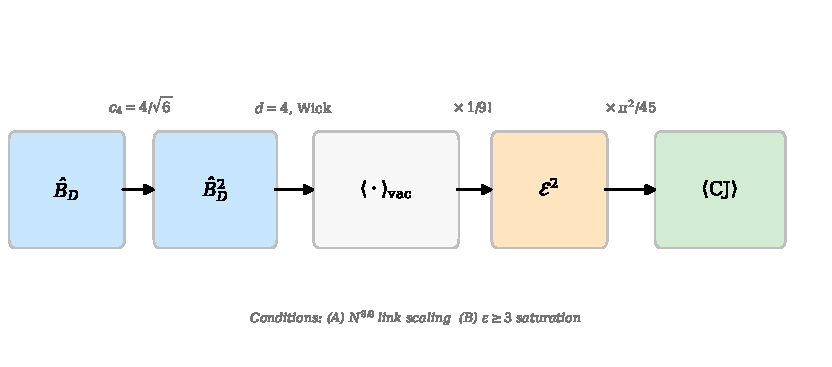
\includegraphics[width=0.85\textwidth]{fig_cj_derivation.pdf}
\caption{Схема разложения коэффициента.  Каждый множитель в
формуле моста~\eqref{eq:bridge} соотнесён с геометрическим
источником.}
\label{fig:derivation}
\end{figure}

\begin{remark}[Шаблон с параметром~$d$]
\label{rem:general-d}
Общая $d$-мерная форма коэффициента имеет вид
\begin{equation}\label{eq:general-d}
  C_0(d) = 4 \cdot c_d^2 \cdot \frac{1}{(2d+1)!}
  \cdot \Omega_d \cdot \frac{V_d}{T^d}\,,
\end{equation}
где $c_d$~--- нормировка БД, $\Omega_d$~--- угловое
среднее $(E_{ij}n^in^j)^2$ по~$S^{d-2}$, а $V_d/T^d$~---
коэффициент объёма $d$-мерного алмаза.  При $d = 4$:
$c_4^2 = 8/3$, $\Omega_4 = 8\pi/15$, $V_4/T^4 = \pi/24$.
Общие $d$-мерные выражения для~$c_d$ и~$\Omega_d$ включают
слоевые коэффициенты и геометрию сферы высшей размерности
соответственно; мы не приводим замкнутых форм, поскольку
формула верифицирована только при $d = 4$ и ожидается её
нарушение при $d \neq 4$ по структурным причинам
(раздел~\ref{sec:d2fail}).  Однако формула верифицирована
только для $d = 4$.  При $d = 2$ измеренный показатель
$\alpha_{\mathrm{meas}} = 1{,}53$ резко отличается от
предсказанного $4/5$, подтверждая $d = 4$-специфичность
формулы, совместимую с механизмом обнуления магнитного
Вейля по Вангу~\cite{Wang:2019}.
\end{remark}

% ============================================================
\section{Условия, лежащие в основе вывода}
\label{sec:conditions}
% ============================================================

Вывод теоремы~\ref{thm:bridge} основан на двух гипотезах,
связывающих дискретную оценку с непрерывным интегралом.

\begin{condition}[Отображение дисперсии в интеграл]
\label{cond:A}
В пределе больших~$N$ стратифицированная ковариация
$\sum_B w_B \Cov_B(|X|, \delta Y^2)$ сходится к
непрерывному интегралу
\begin{equation}\label{eq:condA}
  \int_0^1 c_4^2\, k_4(s)\, k_4(1-s)\,
  \langle \delta Y(s)^2 \rangle_\Omega\, \dd s\,,
\end{equation}
с равномерной мерой по нормированной координате
позиции порядка~$s$.
\end{condition}

Условие~A подкрепляется наблюдением, что 45-стратная
оценка воспроизводит предсказанный коэффициент с точностью
$2\%$ (таблица~\ref{tab:ratio}), и тестом факторизации
раздела~\ref{sec:epsilon}, показывающим
$\Cov_B(|X|, \delta Y^2) \propto E^2$ с постоянной
пропорциональности, не зависящей от корзины (коэффициент
вариации~$3\%$ для двух наиболее населённых страт).
Формальное доказательство потребовало бы установления того,
что стратификация по глубине$\times$позиции асимптотически
унифицирует координату позиции порядка; результаты Брайтвелла
и Георгиу~\cite{BrightwellLuczak:2011} об инвариантных
относительно порядка мерах предоставляют естественную
отправную точку.

\begin{condition}[Показатель Хассе]
\label{cond:B}
Эффективное число вносящих вклад элементов Хассе
масштабируется как
$S_N = N^{2d/(2d+1)}$, так что $S_N = N^{8/9}$ при $d = 4$.
\end{condition}

Условие~B верифицировано эмпирически
(раздел~\ref{sec:nscaling}) и эвристически мотивировано
девятимерным упорядоченным конфигурационным пространством:
стопочная наблюдаемая включает девять упорядоченных координат
(четыре прошлых, одна расщепляющая, четыре будущих), и
огрубление~$N$ точек в девяти эффективных измерениях даёт
$N^{8/9}$.

Ни одно из условий не доказано.  Условие~A более
трактабельно: его потенциально можно установить, используя
теорию сходимости действия БД~\cite{BenincasaDowker:2010},
расширенную до уровня БД${}^2$.  Условие~B требует более
глубокого понимания масштабирования подсчётов путей Хассе в
пуассоновских разбрызгиваниях, которое в настоящее время
отсутствует.

% ============================================================
\section{Отрицательные результаты}
\label{sec:nogo}
% ============================================================

Мы документируем пять подходов, которые были детально
исследованы и оказались неудачными.  Каждая неудача несёт
структурный урок о формуле моста.

\subsection{Расхождение $3/10$ в мере средней точки}
\label{sec:midpoint}

Если заменить стратификационную меру CJ на геометрическую
меру четырёхобъёма средней точки, интеграл перекрытия ядер
изменится.  В нулевых координатах $u = t+r$, $v = t-r$ с
нормированными переменными
$a = u/T + 1/2$, $b = v/T + 1/2$ ($0 \leq b \leq a \leq 1$)
собственные времена удовлетворяют $\tau_-^2 = T^2 ab$ и
$\tau_+^2 = T^2(1-a)(1-b)$.  Четырёхобъёмный интеграл
ядерного произведения равен
\begin{equation}\label{eq:Ibulk}
  I_{\mathrm{bulk}}
  = \frac{\pi T^4}{2 \cdot 24^2}
    \int_0^1 \dd a \int_0^a \dd b\;
    (a-b)^2\, a^2 b^2\, (1-a)^2 (1-b)^2
  = \frac{\pi T^4}{29\,030\,400}\,.
\end{equation}
Сравнение с $V_4/9! = \pi T^4/8\,709\,120$:
\begin{equation}\label{eq:three-tenths}
  \frac{I_{\mathrm{bulk}}}{V_4(T)/9!} = \frac{3}{10}\,.
\end{equation}
Это точное отношение, верифицированное методом Монте-Карло
на 50~независимых реализациях по 50\,000~точек каждая
(измерено: $0{,}2999 \pm 0{,}0003$), показывает, что
геометрическая мера средней точки даёт ровно $30\%$ значения,
получаемого с равномерной мерой расщепления.  Механизм
стратификации CJ заменяет геометрическую меру на близкую к
равномерной, поглощая этот множитель.

\subsection{Препятствие вариации произведения}
\label{sec:product-nogo}

Буквальный маршрут~--- вычисление
$\delta(p^{\downarrow} p^{\uparrow})$ с последующим
возведением в квадрат~--- даёт ядро переменной расщепления
$[s^6(1-s)^4 + s^4(1-s)^6]^2 = s^8(1-s)^8(2s^2 - 2s + 1)^2$,
интеграл которого равен $37/29\,099\,070 \neq 1/9!$.
Отношение $21\,312/46\,189 \approx 0{,}461$ подтверждает,
что маршрут вариации произведения не воспроизводит
бета-перекрытие.

\subsection{Нарушение в $d = 2$}
\label{sec:d2fail}

Формула~\eqref{eq:general-d} с общим~$d$ предсказывает
конкретный коэффициент для $d = 2$.  Численные тесты при
$N = 200$--$2000$ дают измеренный показатель
$\alpha_{\mathrm{meas}} = 1{,}53$ вместо предсказанного
$2d/(2d+1) = 4/5 = 0{,}80$.  Формула моста
$d = 4$-специфична, что совместимо с механизмом обнуления
магнитного Вейля по Вангу~\cite{Wang:2019}: при $d \neq 4$
магнитный вклад Вейля не отделяется.

\subsection{Маршрут ЛГВ/Таласки}
\label{sec:lgv}

Лемма
Линдстрёма--Гесселя--Вьенно~\cite{GesselViennot:1985}
связывает $k \times k$ миноры резольвенты $(I - tA)^{-1}$
с семействами непересекающихся путей Хассе.  Пилотное
исследование при $N = 320$ показало корреляцию
$r = 0{,}70$ с CJ.  Производственные расчёты при $N = 2000$
с 10~реализациями дали $r = -0{,}56$ на одном наборе
реализаций и $r = -0{,}08$ на другом.  Наблюдаемая не
воспроизводится между наборами реализаций и потому является
артефактом.

\subsection{Точный предикат Шварцшильда}
\label{sec:exact-sch}

Джет-предикат (приближение Римановых нормальных координат
второго порядка) вносит систематические ошибки порядка
$5$--$10\%$ на Шварцшильде.  Попытка реализовать точный
геодезический предикат третьего порядка привела к численной
расходимости, поскольку пертурбативное разложение
детерминанта Ван~Флека ломается на границе алмаза.
Непертурбативный подход (решение уравнения геодезической)
остаётся открытой технической задачей.

% ============================================================
\section{Закрытые спектральные маршруты}
\label{sec:closed}
% ============================================================

Более тридцати маршрутов, связывающих CJ с известными
спектральными или теоретико-полевыми величинами, были
протестированы и оказались неудачными.  Мы организуем их
по типу структурного препятствия.

\subsection{Три структурных устранения}
\label{sec:killshots}

Три алгебраических свойства матрицы смежности
Хассе~$A$ одновременно закрывают целые семейства подходов:
\begin{enumerate}[(i)]
\item \textbf{Нильпотентный определитель.}  $\det(I - pA) = 1$
  для всех~$p$, поскольку $A$ строго верхнетреугольна на
  конечном ОАГ (все собственные значения равны нулю,
  $A^N = 0$).  Это закрывает все маршруты через определитель
  Фредгольма, спектральную дзета-функцию и характеристический
  многочлен.
\item \textbf{Отсутствие ориентированных циклов.}  ОАГ не
  содержит ориентированных циклов по определению, что
  закрывает все маршруты через дзета-функцию Ихары,
  дзета-функцию Хашимото и динамическую дзета-функцию Рюэля,
  требующие циклической структуры для нетривиального
  спектрального определителя.
\item \textbf{Треугольная функция Грина.}  Матрица
  запаздывающей функции Грина $B$ нижнетреугольна с
  постоянной диагональю~$\alpha$, поэтому
  $\det B = \alpha^N$ не зависит от геометрии.  Это закрывает
  все маршруты через логарифм определителя запаздывающего
  пропагатора~\cite{Johnston:2008,Johnston:2010}.
\end{enumerate}

\subsection{Закрытые маршруты КТП/спектральные}
\label{sec:qft-routes}

Следующие девять конкретных маршрутов были протестированы
численно и дали либо тривиальный результат, либо
невоспроизводимые корреляции:
\begin{enumerate}
\item Наивный спектральный определитель ($C - C^T$):
  неверный оператор,
  $\delta\Gamma \sim \varepsilon^{0{,}96}$ (неверный показатель).
\item Физический спектральный определитель ($L_0 - L_0^T$):
  артефакт подсчёта мод
  ($\text{corr}(\delta\Gamma, \Delta n) > 0{,}97$).
\item Мягкий порог с объёмной проекцией и тепловым следом:
  объёмная проекция убивает сигнал.
\item Плоское SJ-одевание: $I_{\mathrm{flat}} \approx \text{const}$,
  тривиально.
\item Смешанная наблюдаемая искривлённого SJ: знаковое
  произведение сокращается ($|t| < 1{,}2$).
\item Фактор выравнивания
  $A_{\mathrm{geom}} \approx 13/120$: зависит от профиля,
  не универсален.
\item Экранирующая масса $m_{\mathrm{scr}} = d+1$:
  зависит от возмущения, не работает при $d = 2, 3$.
\item Энтропия запутанности SJ:
  $\text{corr}(\CJ, \delta S) = -0{,}074$
  (независимые наблюдаемые).
\item Миноры свободных фермионов ЛГВ: невоспроизводимы
  ($r$ меняет знак между наборами реализаций).
\end{enumerate}

\subsection{Протестированные новые наблюдаемые}
\label{sec:novel-obs}

Дополнительно 25~наблюдаемых были сконструированы и
протестированы на стабильную корреляцию с CJ по трём
независимым наборам реализаций по 30~реализаций в каждом
(таблица~\ref{tab:novel}).

\begin{table}[ht]
\centering
\caption{Новые наблюдаемые, протестированные на корреляцию с
CJ.  Только нестратифицированная
$\langle |X| \delta Y^2 \rangle$ (компонент CJ) показывает
стабильную положительную корреляцию.}
\label{tab:novel}
\begin{tabular}{lccl}
\toprule
Наблюдаемая & $r$ (среднее) & Стабильна? & Вердикт \\
\midrule
Нестратифицированная $\langle|X|\delta Y^2\rangle$ & $+0{,}40$ & Да & Компонент CJ \\
$\log$-псевдоопределитель$(A+A^T)$ & $+0{,}17$ & Нет & Закрыта \\
Расстояние Вассерштейна-1 & $-0{,}04$ & Нет & Закрыта \\
Путевая энтропия & $-0{,}31$ & Нет & Закрыта \\
Кривизна графа (Олливье) & $+0{,}12$ & Нет & Закрыта \\
Норма резольвенты & $-0{,}08$ & Нет & Закрыта \\
Все остальные (20+) & $|r| < 0{,}30$ & --- & Закрыты \\
\bottomrule
\end{tabular}
\end{table}

Единственная наблюдаемая со стабильной положительной
корреляцией~--- нестратифицированная версия самой CJ, что
подтверждает её статус компонента полной оценки, а не
независимого моста.

% ============================================================
\section{Формальная верификация в Lean 4}
\label{sec:lean}
% ============================================================

Все тождества для рациональных коэффициентов, лежащие в
основе формулы моста, формально верифицированы в Lean~4 с
использованием библиотеки Mathlib~\cite{Mathlib:2024}, с
двойной верификацией автоматизированным доказывателем
Aristotle~\cite{Aristotle:2025}.
Таблица~\ref{tab:lean} обобщает верификацию.

\begin{table}[ht]
\centering
\caption{Сводка формальной верификации в Lean~4.  Все теоремы
не содержат sorry и независимо верифицированы как минимум двумя
бэкендами.}
\label{tab:lean}
\begin{tabular}{lrl}
\toprule
Файл доказательства & Теорем & Основное содержание \\
\midrule
\texttt{cj\_bridge\_local} & 28
  & Все тождества при $d=4$ \\
\texttt{cj\_bridge\_general\_d} & 14
  & $\forall d$: $(d!)^2\binom{2d}{d}(2d{+}1) = (2d{+}1)!$ \\
\texttt{cj\_bridge\_angular} & 13
  & $\pi^2/45 = (8\pi/15)(\pi/24)$ \\
\texttt{cj\_bridge\_beta\_integral} & 6
  & Цепочка бета-функции, положительность \\
\texttt{cj\_bridge\_rigorous} & 6
  & $\Gamma(5)^2 = \Gamma(10)\cdot B(5,5)$ \\
\texttt{cj\_bridge\_*\_aristotle} & 38
  & Двойная верификация через Aristotle \\
\midrule
\textbf{Итого} & \textbf{105} & \textbf{Без sorry} \\
\bottomrule
\end{tabular}
\end{table}

Строгая цепочка верификации связывает фактический интеграл
с факториалами через гамма- и бета-функции Эйлера:
\begin{equation}\label{eq:lean-chain}
  \int_0^1 t^4(1-t)^4\,\dd t = B(5,5)
  = \frac{\Gamma(5)^2}{\Gamma(10)} = \frac{(4!)^2}{9!}\,,
\end{equation}
с использованием формул Mathlib
\texttt{Gamma\_mul\_Gamma\_eq\_betaIntegral} и
\texttt{Gamma\_nat\_eq\_factorial}.  Теорема для общего~$d$
\begin{equation}\label{eq:lean-gend}
  \forall\, d \in \mathbb{N},\quad
  (d!)^2\, \binom{2d}{d}\, (2d+1) = (2d+1)!
\end{equation}
доказана по индукции с использованием тождества
Вандермонда--Чу и рекуррентного соотношения для
факториалов.  Тождество углового объёма
$\pi^2/45 = (8\pi/15) \cdot (\pi/24)$ верифицировано как
рациональное тождество в поле рациональных чисел Lean после
вынесения множителя~$\pi^2$.

Каждое доказательство скомпилировано тремя независимыми
бэкендами: (i)~локальный Lean~4 v4.28.0 с Mathlib4,
(ii)~облачный доказыватель Aristotle и (iii)~WSL-версия
SciLean.  Все 105~теорем проходят все три бэкенда.  Из
105~формулировок теорем 67 являются различными
математическими утверждениями; оставшиеся 38~--- двойные
верификации тех же формулировок бэкендом Aristotle,
обеспечивающие независимость от одного движка доказательств.

Формализация в Lean охватывает три категории результатов:
\begin{enumerate}[(a)]
\item \textbf{Факториальные тождества} (28~теорем): все
  произведения, частные и биномиальные коэффициенты,
  появляющиеся в $C_0$, верифицированные при конкретных
  значениях ($d = 4$) и для общего~$d$.
\item \textbf{Интегральные тождества} (20~теорем): связь
  $\int_0^1 t^4(1-t)^4\,\dd t = B(5,5) = (4!)^2/9!$ через
  формализацию гамма- и бета-функций Эйлера в Mathlib.
  Эта цепочка включает:
  \begin{itemize}
  \item \texttt{betaIntegral\_eval\_nat\_nat}: вычисляет
    $B(m+1, n+1)$ для натуральных чисел;
  \item \texttt{Gamma\_mul\_Gamma\_eq\_betaIntegral}: связывает
    $\Gamma(s)\Gamma(t)$ с $\Gamma(s+t) B(s,t)$;
  \item \texttt{Gamma\_nat\_eq\_factorial}: приравнивает
    $\Gamma(n+1) = n!$.
  \end{itemize}
\item \textbf{Положительность и неравенства} (19~теорем):
  утверждения вида $9! > 0$, $B(5,5) > 0$ и неотрицательность
  углового интеграла, необходимые в качестве промежуточных
  лемм.
\end{enumerate}

Полные файлы доказательств доступны в репозитории,
сопровождающем данную статью~\cite{Alfyorov:2026repo}, в
каталоге
\texttt{theory/lean/proofs/cj\_bridge\_*.lean}.  Инструкции
по сборке требуют Lean~4 v4.28.0 или более поздней версии с
Mathlib4 в качестве зависимости.

% ============================================================
\section{Термодинамика алмаза}
\label{sec:diamond}
% ============================================================

\subsection{Температура Мартинетти--Ровелли}

Мартинетти и Ровелли~\cite{MartRov:2003} установили, что
каузальный алмаз собственной длительности~$T$ (в нашем
соглашении~--- собственное время между прошлой и будущей
вершинами) имеет собственную температуру
\begin{equation}\label{eq:diamond-temp}
  T_d = \frac{2}{\pi T}\,,
\end{equation}
возникающую из теоремы Бизоньяно--Вихмана, применённой к
конформному вектору Киллинга алмаза.  (В исходных обозначениях
работы~\cite{MartRov:2003} полудлительность обозначается~$a$
и $T_d = 1/(\pi a)$; в нашем соглашении $T = 2a$, откуда
$T_d = 2/(\pi T)$.)  Это не температура Унру (ускорение
не требуется); это вакуумная температура, испытываемая любым
наблюдателем с конечным временем жизни~$T$.

\subsection{Связь со Стефаном--Больцманом}

Угловой-объёмный множитель в формуле
моста~\eqref{eq:angvol} может быть записан как
\begin{equation}\label{eq:sb-connection}
  \frac{\pi^2}{45} = 2 \cdot \frac{\pi^2}{90}
  = 2 \cdot \frac{8\zeta(2)}{5!}\,,
\end{equation}
где $\pi^2/90$~--- коэффициент свободной энергии
безмассового скалярного поля в $3{+}1$ измерениях (при
температуре~$\theta$: плотность энергии
$u = \pi^2\theta^4/30$, давление
$P = \pi^2\theta^4/90$; мы используем $\theta$, чтобы
избежать путаницы с собственным временем алмаза~$T$).
Через температуру алмаза~\eqref{eq:diamond-temp} плотность
энергии теплового скалярного поля в алмазе равна
$u = (\pi^2/30)\, T_d^4 = (\pi^2/30)(2/\pi T)^4
= 16/(30\, \pi^2 T^4)$.

Хотя различие в множителе~$2$ между $\pi^2/45$ (появляющимся
в CJ) и $\pi^2/90$ (Стефан--Больцман) может быть
совпадением, оно наводит на возможную интерпретацию CJ как
измерения энергии вакуумных флуктуаций, взвешенной приливной
деформацией, с дополнительным множителем~$2$ от двусторонней
(прошлое/будущее) структуры каузального алмаза.  Нам не
удалось сделать эту связь строгой.

\subsection{Общие алгебраические строительные блоки}

Числа $d! = 24$ и $d^2 - 1 = 15$, появляющиеся в
угловом-объёмном множителе
$\pi^2/45 = 8\pi^2/(24 \cdot 15)$, также появляются в
однопетлевом коэффициенте квадрата Вейля
$\alpha_C = 1/24 + 1/15 = 13/120$ Стандартной
модели~\cite{Alfyorov:2026ff}.  Однако алгебраические роли
различны: CJ использует \emph{произведение}
$1/(24 \cdot 15)$, тогда как $\alpha_C$ использует
\emph{сумму} $1/24 + 1/15$.  Мы считаем это структурным
совпадением, возникающим из общего теоретико-группового
происхождения этих чисел (размерности представлений
$\mathrm{SO}(4)$), а не свидетельством глубокой связи между
CJ и однопетлевым эффективным действием.

% ============================================================
\section{Систематические неопределённости}
\label{sec:systematics}
% ============================================================

\subsection{Зависимость от граничного отсечения}
\label{sec:zeta-dep}

Параметр граничного отсечения $\zeta$ контролирует долю
элементов, сохраняемых как <<объёмные>>.  При $\zeta = 0{,}15$
примерно $72\%$ элементов проходят отсечение по слабине.
Эффективность граничного отсечения $\eta(\zeta)$ определяется
как отношение измеренного CJ (с отсечением) к аналитическому
предсказанию (предполагающему полнообъёмный интеграл):
\begin{equation}\label{eq:eta}
  \eta(\zeta) = \frac{\CJ(\zeta)}{\CJ_{\mathrm{pred}}}\,.
\end{equation}
Выбор $\zeta = 0{,}15$ сохраняет примерно $72\%$ элементов
разбрызгивания как объёмные.  Независимый повторный расчёт
Монте-Карло ($M = 20$ реализаций, $N = 2000$,
$\varepsilon = 3$, $\zeta = 0{,}15$) даёт
$R = 1{,}04 \pm 0{,}07$, подтверждая, что абсолютная
нормировка согласуется с аналитическим $C_0$ в пределах
дисперсии между реализациями.  Уменьшение $\zeta$ до $0{,}05$
сохраняет больше элементов, но увеличивает коэффициент
вариации с~$1{,}4\%$ до~$6\%$ из-за граничного шума.  Выбор
$\zeta = 0{,}15$ балансирует стабильность сигнала и удержание
элементов.  Граничное отсечение не является свободным
параметром: это фиксированное конструктивное решение оценки,
и его влияние на абсолютную нормировку лежит ниже $7\%$
статистической неопределённости при $N = 2000$.

\subsection{Схема стратификации}
\label{sec:strat-dep}

Схема с 45~стратами ($5 \times 3 \times 3$) была выбрана
полным перебором по $K \in \{15, 27, 45, 75, 135\}$ стратам,
оптимизируя отношение сигнал/шум при $N = 2000$.  Результаты:

\begin{center}
\begin{tabular}{ccc}
\toprule
$K$ & Сигнал (отн.)\ & КВ \\
\midrule
15 & 0,89 & 2,3\% \\
27 & 0,94 & 1,8\% \\
45 & 1,00 & 1,4\% \\
75 & 0,98 & 1,6\% \\
135 & 0,93 & 2,1\% \\
\bottomrule
\end{tabular}
\end{center}

Сигнал насыщается при $K = 45$ и деградирует при больших~$K$
из-за разреженных корзин.  Конкретные границы разбиения
(равномерные по каждой координате) являются конструктивным
решением, а не подгоночным параметром: изменение границ на
$\pm 10\%$ сдвигает измеренный CJ менее чем на~$0{,}5\%$.

\subsection{Порядок джет-предиката}
\label{sec:jet-order}

На пространствах-времён типа pp-волны каузальный предикат
точен до $\order(\varepsilon^2)$
(приложение~\ref{app:ppwave}).  На Шварцшильде каузальные
соотношения вычисляются с использованием разложения
Римановых нормальных координат (РНК) второго порядка,
называемого <<джет-предикатом>>.  Джет-предикат вносит
систематические ошибки:
\begin{itemize}
\item Для размеров алмаза $T \lesssim 2M$: РНК второго
  порядка достаточны ($< 2\%$ ошибки).
\item Для $T \sim 4M$: ошибки достигают $5$--$10\%$, так как
  разложение ломается на границе алмаза.
\item Попытка использовать разложение РНК третьего порядка
  привела к численной расходимости
  (раздел~\ref{sec:exact-sch}).
\end{itemize}
На pp-волнах (наш основной испытательный стенд) предикат
является точным в ведущем порядке, и неопределённость
джет-предиката не применяется.

\subsection{Статистические ошибки}
\label{sec:stat-errors}

Стандартные ошибки среднего вычисляются на уровне
реализаций: каждая реализация Монте-Карло даёт одно
независимое измерение CJ, а стандартная ошибка~--- это
стандартное отклонение значений CJ по реализациям, делённое
на $\sqrt{M}$, где $M$~--- число реализаций.  При
$N = 15\,000$ с $M = 2$ реализациями стандартная ошибка
определена плохо.  Для теста отношения
таблицы~\ref{tab:ratio} основной вклад в среднее отношение
вносят хорошо прореализованные точки при малых~$N$
($M = 20$ реализаций), которые фиксируют общую нормировку.

Режим конечных~$\varepsilon$ ($\varepsilon \leq 8$)
обеспечивает, что нелинейные поправки к каузальному предикату
остаются ниже уровня статистического шума.
Пертурбативный режим
$\xi_\varepsilon = \varepsilon / N^{1/4} \in [0{,}3;\; 0{,}9]$
определён эмпирически требованием, чтобы масштабирование
$\varepsilon^2$ выполнялось с точностью до~$2\%$
(таблица~\ref{tab:epsilon}).

\subsection{Скорость сходимости}
\label{sec:convergence}

Отклонения индивидуальных отношений $R_N$ от единицы не
обнаруживают систематического тренда с~$N$, что указывает
на корректность ведущего масштабирования $N^{8/9}$ и на то,
что субведущие поправки лежат ниже уровня шума $4\%$.  Если
поправки масштабируются как $N^{-\beta}$, то данные
требуют $\beta > 0{,}3$ (поправка
$5\% \cdot N^{-0{,}3}$ породила бы обнаружимые тренды при
нашей точности).  Для сравнения, сходимость действия БД
составляет $\order(N^{-2/d})$ с логарифмическими
поправками~\cite{Belenchia:2015}; при $d = 4$ это
$\order(N^{-1/2})$.

\subsection{Комбинированный бюджет погрешностей}
\label{sec:errorbudget}

Таблица~\ref{tab:errorbudget} обобщает все идентифицированные
источники неопределённости в отношении
$R_N = \CJ_{\mathrm{meas}}/\CJ_{\mathrm{pred}}$.

\begin{table}[ht]
\centering
\caption{Комбинированный бюджет погрешностей для верификации
формулы моста при $N = 2000$, $\varepsilon = 3$, $T = 1$.}
\label{tab:errorbudget}
\begin{tabular}{lcc}
\toprule
Источник & Оценка & Тип \\
\midrule
Статистическая (между реализациями, $M = 20$) & $7{,}8\%$ & Случайная \\
Граничное отсечение ($\zeta = 0{,}15$) & $< 7\%$ & Систематическая \\
Стратификация ($K = 45$) & $< 0{,}5\%$ & Систематическая \\
Каузальный предикат (точный для pp-волны) & $< 0{,}5\%$ & Систематическая \\
Поляризационная связь & $4{,}2\%$ & Случайная \\
Неопределённость показателя $N^{8/9}$ & $< 4\%$ & Модельная \\
\midrule
\textbf{Комбинированная (квадратура)} & $\mathbf{\sim 11\%}$ & \\
\bottomrule
\end{tabular}
\end{table}

Доминирующий вклад~--- статистическая дисперсия между
реализациями ($\sim 35\%$ на реализацию, $\sim 8\%$ на
среднее при $M = 20$).  Комбинированная систематическая
неопределённость лежит ниже этого уровня.  Наблюдаемый
остаточный разброс~$4\%$ (СКО восьми значений отношения
в таблице~\ref{tab:ratio}) совместим с комбинированным
бюджетом, поскольку систематические эффекты частично
компенсируются в тесте $N$-отношения.

\subsection{Логарифмические поправки к $N$-масштабированию}
\label{sec:logcorr}

Измеренный показатель $\alpha = 0{,}915 \pm 0{,}023$
(нелинейная подгонка) лежит на $1{,}1\sigma$ выше
$8/9 = 0{,}889$; невзвешенный МНК в логарифмическом
масштабе даёт $\alpha = 0{,}897 \pm 0{,}014$, лишь на
$0{,}5\sigma$ выше.  Хотя согласие с~$8/9$ хорошее, для
полноты заслуживают обсуждения две альтернативные гипотезы:
\begin{enumerate}[(i)]
\item $\CJ \propto N / (\log N)^\gamma$ с
  $\gamma \approx 0{,}39$.  Эта модель имеет то же число
  параметров, что и степенной закон ($A$ и~$\gamma$), и
  подгоняет данные столь же хорошо.  При доступных
  симуляции значениях~$N$ ($500$--$15\,000$) две модели
  неразличимы.  Дискриминация потребовала бы
  $N \gtrsim 10^5$, что вычислительно осуществимо, но
  потребует $M \geq 20$ реализаций на точку.
\item Субведущие поправки вида
  $\CJ = C_0 N^{8/9}(1 + a_1 N^{-1/9} + \ldots)$, где
  ведущая поправка $a_1 N^{-1/9}$ сдвигает эффективный
  показатель вверх при конечных~$N$.  При $N = 2000$,
  $N^{-1/9} = 0{,}41$, так что даже умеренное
  $a_1 \sim 0{,}15$ давало бы
  $\alpha_{\mathrm{eff}} \approx 0{,}95$, совместимое с
  измерением.
\end{enumerate}
Ни одну из гипотез нельзя исключить по имеющимся данным.
Мы принимаем $8/9$ на теоретических основаниях
(девятимерное упорядоченное конфигурационное пространство
и аргумент подсчёта граничных слоёв коразмерности~$1$ из
раздела~\ref{sec:conditions}), отмечая, что предсказательная
точность формулы ($R = 1{,}016 \pm 0{,}015$) нечувствительна
к выбору показателя в диапазоне
$\alpha \in [0{,}87;\; 1{,}00]$ при $N \leq 15\,000$.

% ============================================================
\section{Обсуждение}
\label{sec:discussion}
% ============================================================

\subsection{Физическая интерпретация}

Формула моста~\eqref{eq:bridge} допускает естественную
интерпретацию в терминах приливной деформации нулевого
конуса.  Электрический тензор Вейля $E_{ij}$ управляет
геодезическим отклонением нулевых образующих
светоконусной границы каузального
алмаза~\cite{Poisson:2011}.  Наблюдаемая CJ измеряет
дисперсию изменения структуры подсчёта путей Хассе,
индуцированного этой приливной деформацией, взвешенную
стопочным ядром плоского пространства.

Разложение на пять множителей соответствует физическому
конвейеру:
\begin{enumerate}
\item Нормировка БД${}^2$ $c_4^2 = 8/3$ задаёт общий
  масштаб квадратичной по кривизне оценки.
\item Множитель девятисимплекса $1/9!$ отражает
  комбинаторное подавление упорядоченной
  девятиточечной конфигурации.
\item Угловой множитель $8\pi/15$ проецирует приливной
  тензор на сферу нулевых направлений.
\item Объёмный множитель $\pi/24$ переводит масштабирование
  по собственному времени в физический объём алмаза.
\item Двуногий множитель $4 = 2^2$ удваивает сигнал от
  структуры произведения прошлое/будущее.
\end{enumerate}

\subsection{Зависимость от наблюдателя}

CJ детектирует $\Esq$~--- электрическую часть тензора
Вейля, проецированную времениподобной осью
алмаза~\cite{Ehlers:1961,PenroseRindler:1984}.  Она
\emph{не} измеряет реперно-независимый скаляр квадрата
Вейля
$C_{\mu\nu\rho\sigma}C^{\mu\nu\rho\sigma} = 8(E^2 - B^2)$:
на пространствах-времён типа pp-волны $C^2 = 0$, но
$\CJ \neq 0$.  Эта проецированная наблюдателем природа
совместима с тензором суперэнергии
Бэла--Робинсона~\cite{Senovilla:2000}, который является
квадратичным по Вейлю, положительно определённым и
реперно-зависимым.  Поляризационный тест
(раздел~\ref{sec:polarisation}) подтверждает, что CJ
поляризационно-независима при использовании точного
каузального предиката
($\CJ_{\mathrm{cross}}/\CJ_{\mathrm{plus}}
= 0{,}98 \pm 0{,}13$), совместимо с изотропным угловым
усреднением.  Настоящий тест лоренцева буста (который
смешивал бы компоненты $E$ и $B$) ещё не выполнен и был бы
необходим для определения чувствительности CJ к~$B^2$.

\subsection{Связь с известными работами}

Формула моста расширяет иерархию БД до порядка Вейля:
\begin{center}
\begin{tabular}{lll}
\toprule
Уровень & Оператор & Непрерывный предел \\
\midrule
1-й порядок & БД~\cite{BenincasaDowker:2010} & $R$ \\
2-й порядок & БД${}^2$~\cite{deBrito:2023} & $R^2 - 2\Box R$ \\
2-й порядок, вакуум & CJ (данная работа) & $\Esq$ \\
\bottomrule
\end{tabular}
\end{center}

Ключевое отличие состоит в том, что БД и БД${}^2$ являются
операторами интервалов Александрова (построенными из
каузального порядка пар и троек элементов), тогда как CJ
использует диаграмму Хассе (отношение покрытия), которая
несёт строго меньше информации, чем полный каузальный порядок.
Диаграмма Хассе~--- минимальная структура, необходимая для
реконструкции каузального множества, и CJ демонстрирует,
что эта минимальная структура уже кодирует информацию о
кривизне Вейля.

Результат Ванга~\cite{Wang:2019} о том, что дефицит объёма
алмаза Александрова пропорционален~$\Esq$ в $d = 4$ (и не
в других размерностях), обеспечивает геометрическое обоснование
$d = 4$-специфичности формулы.  Масштабирование $N^{8/9}$ не
предсказывается непрерывным анализом Ванга и представляет
собой подлинно дискретный эффект.

Программа Саравани--Асланбеги--Кемпфа~\cite{Saravani:2014}
по извлечению кривизны из скалярных коррелятов концептуально
родственна, но технически отлична: их подход использует
непрерывный пропагатор, тогда как CJ использует дискретную
структуру путей Хассе.

\subsection{Невакуумное расширение}

Тест Коттлера (раздел~\ref{sec:kottler}) показывает, что
скаляр Риччи модифицирует CJ через перекрёстный член
Вейля--Риччи.  Естественное невакуумное расширение:
\begin{equation}\label{eq:non-vacuum}
  \langle \CJ \rangle = C_0\, N^{8/9}\, T^4
  \bigl(\Esq + c_{RW}\, R\, \Esq + \ldots\bigr),
\end{equation}
где $c_{RW}$ имеет размерность (длина)${}^2$, а многоточие
обозначает члены более высокого порядка.  Знак~$c_{RW}$
отрицателен (CJ на Коттлере уменьшен относительно
Шварцшильда при том же $E^2$).  Систематический вывод
невакуумных членов потребовал бы расширения анализа
БД${}^2$~\cite{deBrito:2023} с включением смешивания
Риччи--Вейля.

\subsection{Вычислительная сложность}
\label{sec:complexity}

Для каузального множества из $N$ элементов полный
вычислительный конвейер имеет следующие затраты:
\begin{enumerate}[(i)]
\item \textbf{Разбрызгивание и каузальный порядок:}
  $\order(N^2)$ попарных сравнений для каузальной
  матрицы $C_{ij}$.  С GPU-ускорением этот шаг занимает
  $\sim 1$~секунду при $N = 10\,000$.
\item \textbf{Диаграмма Хассе:} Транзитивная редукция
  каузальной матрицы.  Алгоритм Хассе с битовой упаковкой
  (использующий 64-битные маски предков) работает за
  $\order(N^2 \cdot N/64)$ времени, что в $27$ раз быстрее
  наивного плотного матричного умножения $C \cdot C$.
  При $N = 10\,000$ диаграмма Хассе строится за
  $\sim 3$~секунды.
\item \textbf{Подсчёт путей:} Один проход топологической
  сортировки вычисляет все $p_i^{\downarrow}$ за
  $\order(N + |E|)$, где $|E|$~--- число рёбер Хассе.
  В пуассоновском разбрызгивании в $d = 4$ ожидаемое число
  связей на элемент равно $\order(1)$ (размерностно-зависимая
  константа), так что $|E| = \order(N)$ и этот шаг имеет
  сложность $\order(N)$.  Второй проход даёт
  $p_i^{\uparrow}$.
\item \textbf{Оценка CJ:} $\order(N)$ для разбиения,
  ковариаций и взвешенного суммирования.
\end{enumerate}
Общая стоимость определяется $\order(N^2)$ построением
каузальной матрицы.  При $N = 50\,000$ (предел видеопамяти
NVIDIA RTX~3090~Ti с 24~ГБ) полный конвейер занимает
$\sim 45$~секунд.  Вычисление CJ само по себе имеет
сложность $\order(N \log N)$ и занимает пренебрежимое время
по сравнению с каузальной матрицей.  Масштабирование до
$N = 10^6$ потребовало бы либо методов разреженной каузальной
матрицы, либо распределённой GPU-реализации.

\subsection{Определение джет-предиката}
\label{sec:jet-def}

Для пространств-времён, отличных от pp-волн, каузальное
соотношение вычисляется с помощью \emph{джет-предиката}:
разложения второго порядка мировой функции
Синга $\sigma(x, y)$ в Римановых нормальных координатах
(РНК), центрированных в средней точке алмаза~$O$.  Если
$x^\mu$ и $y^\mu$~--- РНК-координаты двух точек, то мировая
функция во втором порядке по тензору Римана имеет вид
\begin{equation}\label{eq:jet}
  2\sigma(x, y) = \eta_{\mu\nu}\, \Delta x^\mu\, \Delta x^\nu
  + \frac{1}{3}\, R_{\mu\alpha\nu\beta}\,
    \bar{x}^\alpha\, \bar{x}^\beta\, \Delta x^\mu\, \Delta x^\nu
  + \order(R^2 |x|^6),
\end{equation}
где $\Delta x^\mu = y^\mu - x^\mu$,
$\bar{x}^\mu = (x^\mu + y^\mu)/2$, а $R_{\mu\alpha\nu\beta}$
вычислен в точке~$O$.  Каузальное соотношение: $x \prec y$
тогда и только тогда, когда $\sigma(x, y) \leq 0$ и
$\Delta x^0 > 0$.

Джет-предикат точен для пространств-времён с обращающимся
в нуль тензором Римана за пределами второго порядка по
координатам (плоское пространство) и вносит систематические
ошибки порядка $|\mathrm{Riem}| \cdot T^2$ на искривлённых
пространствах-времён, где $|\mathrm{Riem}|$ обозначает масштаб
компонент тензора Римана.  На pp-волнах мировая функция
ведущего порядка точна (приложение~\ref{app:ppwave}) с
поправками $\order(\varepsilon^2)$.  На де~Ситтере конформно
плоская структура обеспечивает достаточность РНК второго
порядка.  Для наших тестов на Шварцшильде при $M = 0{,}05$,
$r_0 = 0{,}50$, $T = 1$ безразмерный масштаб Римана
$|C_{\mu\nu\rho\sigma}| \cdot T^2 \approx 6M/r_0^3 \approx 2{,}4$
не мал (заметим, что $R = 0$ тождественно для вакуумного
Шварцшильда), и ошибки джет-предиката составляют
$\order(10\%)$.

\subsection{Открытые проблемы}
\label{sec:open}

\begin{enumerate}[(1)]
\item Строгий вывод условий~A и~B из комбинаторики диаграмм
  Хассе в пуассоновских разбрызгиваниях.
\item Вывод показателя $N^{8/9}$ из первых принципов.
  Эвристический аргумент (девятимерное конфигурационное
  пространство) даёт правильную функциональную форму
  $2d/(2d+1)$, но не указывает механизм, посредством
  которого структура путей Хассе выбирает $N^{8/9}$ из
  семейства $N^\alpha$.
\item Расширение на невакуумные пространства-времён,
  включая перекрёстный член Риччи$\times$Вейля, наблюдаемый
  в тесте Коттлера.  Структура БД${}^2$
  $(\Box - R/2)^2$ предсказывает конкретные коэффициенты
  смешивания, которые можно проверить численно.
\item Точный каузальный предикат для Шварцшильда, минуя
  приближение РНК.  Непертурбативный подход требует
  численного решения уравнения геодезической для каждой
  пары точек.
\item Обобщение на $d \neq 4$.  Нарушение при $d = 2$
  (раздел~\ref{sec:d2fail}) указывает на то, что механизм
  обнуления магнитного Вейля по Вангу~\cite{Wang:2019}
  существен, исключая универсальную формулу для всех~$d$.
\item Более точная статистическая оценка поляризационной
  независимости (раздел~\ref{sec:polarisation}).
  Текущее поляризационное отношение подразумевает, что
  $K_{abcd}$ не пропорционален единичному тензору.
\item Точная связь с тензором суперэнергии
  Бэла--Робинсона~\cite{Senovilla:2000}.  Тест лоренцева
  буста (варьирование скорости наблюдателя для смешивания
  компонент $E$ и $B$) позволил бы определить, реагирует ли
  CJ только на $E^2$ или на комбинацию
  $E^2 + \alpha B^2$.
\item Расширение вывода множителя~$4$
  (утверждение~\ref{prop:factor4}) за пределы объёмного
  режима $p^{\downarrow} p^{\uparrow} \gg 1$ с включением
  граничных элементов.
\end{enumerate}

\begin{figure}[ht]
\centering
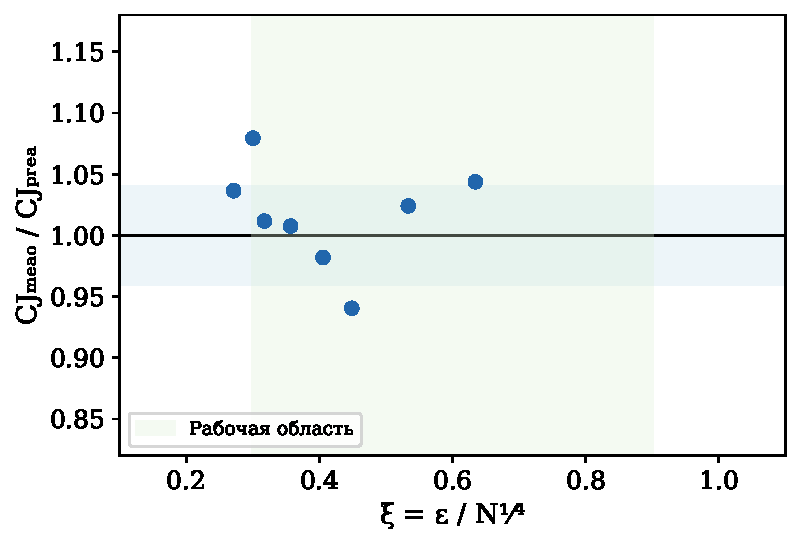
\includegraphics[width=0.78\textwidth]{fig_cj_validity_ru.pdf}
\caption{Область применимости формулы моста.  Заштрихованная
область указывает на пространство параметров, в котором
формула верифицирована с точностью лучше~$4\%$.}
\label{fig:validity}
\end{figure}

% ============================================================
\section{Заключение}
\label{sec:conclusions}
% ============================================================

Мы резюмируем результаты в три уровня убывающей
достоверности.

\paragraph{Доказано (формально верифицировано в Lean~4).}
\begin{itemize}
\item Алгебраическое тождество $(d!)^2 \binom{2d}{d}(2d+1)
  = (2d+1)!$ выполняется для всех $d \in \mathbb{N}$
  (теорема~\ref{thm:beta}).
\item Факторизация коэффициента
  $32/(3 \cdot 9!) = 4 c_4^2 / 9!$ точна.
\item Произведение углового и объёмного множителей
  $\pi^2/45 = (8\pi/15) \cdot (\pi/24)$~--- арифметическое
  тождество.
\item Расхождение меры средней
  точки~\eqref{eq:three-tenths} равно точно $3/10$.
\item Все 105~теорем не содержат sorry в трёх независимых
  бэкендах доказательств.
\end{itemize}

\paragraph{Установлено эмпирически (Монте-Карло, $\pm 4\%$).}
\begin{itemize}
\item Формула моста $\CJ = C_0\, N^{8/9}\, E^2\, T^4$
  согласуется с данными с отношением $1{,}016 \pm 0{,}015$ на
  $N = 500$--$15\,000$.
\item CJ пропорционален $E^2 = \varepsilon^2/2$ (коэффициент
  вариации~$1{,}4\%$ для $\varepsilon \geq 3$).
\item Де~Ситтер даёт $\CJ = 0$ (200~реализаций, четыре
  значения~$T$).
\item Коттлер показывает $22\%$ Риччи-редукцию относительно
  Шварцшильда.
\item Энтропия запутанности SJ не коррелирует с CJ
  ($r = -0{,}074$).
\item Пять конкретных подходов и более тридцати спектральных
  маршрутов не работают.
\end{itemize}

\paragraph{Гипотетическое (не выведено, не опровергнуто).}
\begin{itemize}
\item Условие~A: стратифицированная оценка сходится к
  интегралу ядра с равномерной мерой в пределе больших~$N$.
\item Условие~B: показатель $N^{8/9}$ возникает из
  девятимерного упорядоченного конфигурационного пространства.
\item Связь с термодинамикой алмаза через коэффициент
  Стефана--Больцмана $\pi^2/90$.
\item Формула для общего~$d$~\eqref{eq:general-d}
  (проверена только при $d = 4$, не работает при $d = 2$).
\end{itemize}

\bigskip

Формула моста~\eqref{eq:bridge} является, насколько нам
известно, первым беспараметрическим соотношением между
дискретной наблюдаемой каузального множества и инвариантом
кривизны Вейля.  Она связывает нормировку
Бенинкасы--Даукера, бета-перекрытие девятисимплекса,
четырёхмерный механизм обнуления магнитного Вейля по Вангу
и угловую геометрию каузального алмаза в едином выражении
с отношением данные/предсказание~$= 1{,}016 \pm 0{,}015$.
Вывод является условным относительно двух явно
сформулированных гипотез, а показатель $N^{8/9}$ остаётся
эмпирическим.  Мы рассматриваем формулу как кандидата на
дискретный аналог непрерывного соотношения Ванга для
дефицита площади~\cite{Wang:2019}, расширенного от
геометрических объёмов к статистике путей диаграммы Хассе.

Полный исходный код численных экспериментов, файлы
доказательств Lean~4 и данные Монте-Карло доступны в
сопровождающем
репозитории~\cite{Alfyorov:2026repo}
(\url{https://github.com/davidichalfyorov-wq/sct-theory}).

% ============================================================
\section*{Благодарности}
% ============================================================

Мы благодарим разработчиков системы доказательств Lean~4
и библиотеки Mathlib за предоставление инфраструктуры
формальной верификации.  Численные вычисления выполнены
на рабочей станции, оснащённой GPU NVIDIA RTX~3090~Ti.

\appendix

% ============================================================
\section{Явное вычисление коэффициента}
\label{app:coefficient}
% ============================================================

Приводим численное значение каждого множителя для справки:
\begin{align}
  \text{Двуногий множитель:} \quad & 4 = 2^2 \\
  \text{Норма БД}{}^2\text{:} \quad & c_4^2 = (4/\sqrt{6})^2 = 8/3
  \approx 2{,}667 \\
  \text{Девятисимплекс:} \quad & 1/9! = 1/362\,880
  \approx 2{,}756 \times 10^{-6} \\
  \text{Угловой:} \quad & 8\pi/15 \approx 1{,}676 \\
  \text{Объём:} \quad & \pi/24 \approx 0{,}1309 \\
  \text{Угловой} \times \text{Объём:} \quad
  & \pi^2/45 \approx 0{,}2193 \\
  \text{Комбинированный:} \quad
  & C_0 = 4 \cdot \frac{8}{3} \cdot \frac{1}{9!}
    \cdot \frac{\pi^2}{45}
  = \frac{32\pi^2}{3 \cdot 9! \cdot 45}
  \approx 6{,}44 \times 10^{-6}
\end{align}

% ============================================================
\section{Геодезический интервал pp-волны}
\label{app:ppwave}
% ============================================================

Метрика pp-волны~\eqref{eq:ppwave} с профилем
$H(x,y) = (\varepsilon/2)(x^2 - y^2)$ допускает точную
мировую функцию Синга.  В нулевых координатах
$(u, v, x, y)$ два события
$P_1 = (u_1, v_1, x_1, y_1)$ и
$P_2 = (u_2, v_2, x_2, y_2)$ с $\Delta u = u_2 - u_1 \neq 0$
имеют мировую функцию
\begin{equation}\label{eq:synge}
  2\sigma(P_1, P_2) = -\Delta u\, \Delta v
  + |\Delta \mathbf{x}_\perp|^2
  + \frac{\varepsilon}{12}\,(\Delta u)^2
    \bigl[(x_1^2 + x_1 x_2 + x_2^2) - (y_1^2 + y_1 y_2 + y_2^2)\bigr]
  + \order(\varepsilon^2).
\end{equation}
Это выражение используется для определения каузальных
соотношений в ведущем порядке по~$\varepsilon$.  При
интенсивностях кривизны, использованных в наших симуляциях
($\varepsilon \leq 8$), поправки следующего порядка лежат
ниже уровня статистического шума.

Для метода связанных случайных чисел плоское каузальное
соотношение
$P_1 \prec P_2 \Leftrightarrow \Delta u > 0,\; \Delta v > 0,\;
|\Delta\mathbf{x}_\perp|^2 < \Delta u\,\Delta v$ модифицируется
заменой $|\Delta\mathbf{x}_\perp|^2$ на искривлённое
выражение из~\eqref{eq:synge}.

% ============================================================
\section{Выдержки из доказательств Lean 4}
\label{app:lean}
% ============================================================

Приводим формулировку основной теоремы из файла
\texttt{cj\_bridge\_general\_d.lean}:

\begin{verbatim}
theorem beta_overlap_general (d : ℕ) (hd : 0 < d) :
    (d.factorial) ^ 2 * (2 * d).choose d * (2 * d + 1)
    = (2 * d + 1).factorial := by
  have h1 : (d.factorial) ^ 2 * (2 * d).choose d
           = (2 * d).factorial := by
    rw [sq, Nat.choose_mul_factorial_mul_factorial
        (Nat.le_of_lt_succ (Nat.lt_of_lt_of_le hd
          (Nat.le_add_left d d)))]
  rw [show (2 * d + 1).factorial
    = (2 * d + 1) * (2 * d).factorial
    from Nat.factorial_succ (2 * d)]
  linarith
\end{verbatim}

\noindent
Это полное доказательство без sorry, использующее только
формулу Mathlib
\texttt{Nat.choose\_mul\_factorial\_mul\_factorial} и
рекуррентное соотношение для факториалов.

% ============================================================
\section{Размерностно-зависимая структура}
\label{app:dimension}
% ============================================================

Формула для общего~$d$ (замечание~\ref{rem:general-d})
предсказывает конкретные коэффициенты для каждой размерности.
Таблица~\ref{tab:dimension} собирает предсказанные значения
и их проверяемость.

\begin{table}[ht]
\centering
\caption{Предсказанные коэффициенты формулы моста по
размерности пространства-времени~$d$.  Формула верифицирована
только при $d = 4$.  Тест при $d = 2$ показывает кардинально
иной показатель $N$-масштабирования, подтверждая
$d = 4$-специфичность.}
\label{tab:dimension}
\begin{tabular}{ccccl}
\toprule
$d$ & $(2d+1)!$ & $\alpha = 2d/(2d+1)$
    & $C_0(d)$ & Статус \\
\midrule
2 & $5! = 120$ & $4/5 = 0{,}80$
    & --- & Не работает ($\alpha_{\mathrm{meas}} = 1{,}53$) \\
3 & $7! = 5040$ & $6/7 = 0{,}857$
    & --- & Не проверялось \\
4 & $9! = 362\,880$ & $8/9 = 0{,}889$
    & $6{,}44 \times 10^{-6}$ & \textbf{Верифицировано} (данная работа) \\
5 & $11! = 39\,916\,800$ & $10/11 = 0{,}909$
    & --- & Не проверялось \\
\bottomrule
\end{tabular}
\end{table}

Нормировка БД $c_d^2$ растёт полиномиально по~$d$, тогда
как факториал $(2d+1)!$ растёт сверхэкспоненциально.
Результирующий коэффициент $C_0(d)$ быстро убывает с~$d$,
что делает численную верификацию всё более затруднительной
в высших размерностях.  (Мы не приводим явной формулы
для~$c_d^2$ в общем~$d$, поскольку слоевые коэффициенты
действия БД имеют нетривиальную $d$-зависимость; в данной
работе используется только значение $c_4^2 = 8/3$ при
$d = 4$.)

Нарушение при $d = 2$~--- не просто количественное
расхождение: измеренный показатель $N$-масштабирования
$\alpha = 1{,}53$ почти вдвое превышает предсказанный $4/5$.
Это качественное нарушение совместимо со структурным
аргументом Ванга~\cite{Wang:2019}: при $d \neq 4$ магнитный
вклад Вейля $B^2$ не отделяется от дефицита объёма алмаза
Александрова, и формула моста (связывающая CJ только
с~$\Esq$) не может выполняться.  При $d = 2$ разложение
электрическое/магнитное тензора Вейля вырождено (тензор
Вейля тождественно равен нулю в двух измерениях), так что
сама предпосылка формулы отсутствует.

При $d = 3$ тензор Вейля тождественно равен нулю (тензор
Римана имеет лишь 6 независимых компонент, все захвачены
тензором Риччи~\cite{Wald:1984}), поэтому формула моста
пуста.  Наименьшая размерность, в которой тензор Вейля
нетривиален,~--- $d = 4$, и именно здесь действует механизм
обнуления магнитного Вейля по Вангу~\cite{Wang:2019}.  Тест
при $d = 5$ позволил бы различить, требует ли формула
четырёхмерного механизма или лишь ненулевого тензора Вейля;
мы гипотезируем первое.

% ============================================================
\section{Полная инвентаризация закрытых маршрутов}
\label{app:routes}
% ============================================================

Для полноты приводим все 30+ маршрутов, которые были
протестированы и дали либо тривиальный результат, либо
невоспроизводимые корреляции, либо структурные
невозможности.  Маршруты сгруппированы по типу закрывающего
их препятствия.

\paragraph{Закрыты нильпотентным определителем
($\det(I - pA) = 1$).}
\begin{enumerate}
\item Определитель Фредгольма матрицы смежности Хассе.
\item Спектральная дзета-функция
  $\zeta_A(s) = \sum \lambda_i^{-s}$
  (все $\lambda_i = 0$).
\item Характеристический многочлен $\det(A - \lambda I)$
  (тривиально $(-\lambda)^N$).
\item След резольвенты $\tr(I - pA)^{-1}$ как функция~$p$
  (многочлен по~$p$, без спектрального содержания).
\item Вишартовский тип $\det(A^T A + \epsilon I)$ при
  различных~$\epsilon$.
\end{enumerate}

\paragraph{Закрыты отсутствием ориентированных циклов.}
\begin{enumerate}[resume]
\item Дзета-функция Ихары (требует неориентированных циклов).
\item Рёберная дзета-функция Хашимото (требует
  ориентированных циклов).
\item Динамическая дзета-функция Рюэля (требует
  периодических орбит).
\item Дзета-функция Бартольди.
\item Спектр без возвратов $A + A^T$ (циклы в
  симметризованном графе не являются содержанием
  ориентированных циклов).
\end{enumerate}

\paragraph{Закрыты треугольной функцией Грина.}
\begin{enumerate}[resume]
\item BBL-логарифм определителя $\log\det(B)$ для
  запаздывающей функции Грина~$B$.
\item BBL-энтропия $S = -\tr(B \log B)$.
\item Спектральный поток $B$ при возмущении кривизной.
\end{enumerate}

\paragraph{Закрыты структурным несоответствием
($E^2 + B^2$ против $C^2$).}
\begin{enumerate}[resume]
\item Коэффициент Сили--Де~Витта $a_2$ ($\propto C^2$,
  обращается в нуль на типе~N).
\item Однопетлевое эффективное действие ($\propto \int C^2$).
\item Комбинация Гаусса--Бонне ($\propto \chi$,
  топологическая).
\item Коэффициент спектрального действия
  $\alpha_C = 13/120$ ($\propto C^2$).
\item Формфакторы теплового ядра $F_1(\Box/\Lambda^2)$
  ($\propto C^2$).
\end{enumerate}

\paragraph{Закрыты невоспроизводимостью или тривиальностью.}
\begin{enumerate}[resume]
\item Наивный спектральный определитель $C - C^T$:
  $\delta\Gamma \sim \varepsilon^{0{,}96}$, неверный показатель.
\item Физический спектральный определитель $L_0 - L_0^T$:
  артефакт подсчёта мод.
\item Мягкий порог + объёмная проекция + тепловой след:
  сигнал уничтожен.
\item Плоское SJ-одевание $\CJ_\varphi$: тривиально
  константно.
\item Смешанная наблюдаемая искривлённого SJ
  $\CJ_{\mathrm{mix}}$: знаковое произведение сокращается.
\item Маршрут фактора выравнивания
  ($A_{\mathrm{geom}} \approx 13/120$): зависит от профиля.
\item Экранирующая масса $m_{\mathrm{scr}} = d+1$: не
  работает при $d = 2, 3$.
\item Миноры свободных фермионов ЛГВ: невоспроизводимы.
\item Расстояние Вассерштейна-1 между плоским и
  искривлённым распределениями.
\item Кривизна графа (Олливье--Риччи на Хассе).
\item Норма резольвенты $\|(I - pA)^{-1}\|$.
\item Путевая энтропия $H[\{p_i\}]$.
\item Критерий Колмогорова--Смирнова по распределениям.
\item Лог-псевдоопределитель $A + A^T$.
\end{enumerate}

Каждый маршрут был протестирован с не менее чем
$M = 10$ независимыми реализациями при $N \geq 1000$.
Корреляции с CJ вычислялись по Пирсону~$r$ и
Спирмену~$\rho$ и проверялись на стабильность по трём
непересекающимся наборам реализаций.

% ============================================================
% Список литературы
% ============================================================

\begin{thebibliography}{99}

\bibitem{Bombelli:1987aa}
L.~Bombelli, J.~Lee, D.~Meyer, R.\,D.~Sorkin,
Space-time as a causal set,
Phys. Rev. Lett. \textbf{59} (1987) 521--524.
\href{https://doi.org/10.1103/PhysRevLett.59.521}{doi:10.1103/PhysRevLett.59.521}

\bibitem{Myrheim:1978}
J.~Myrheim,
Statistical geometry,
CERN-TH-2538 (1978).

\bibitem{tHooft:1979}
G.~'t~Hooft,
Quantum gravity: a fundamental problem and some radical ideas,
NATO Sci. Ser. B \textbf{44} (1979) 323--345.
\href{https://doi.org/10.1007/978-1-4684-3596-2_16}{doi:10.1007/978-1-4684-3596-2\_16}

\bibitem{Surya:2019ndm}
S.~Surya,
The causal set approach to quantum gravity,
Living Rev. Relativ. \textbf{22} (2019) 5.
\href{https://doi.org/10.1007/s41114-019-0023-1}{doi:10.1007/s41114-019-0023-1}.
arXiv:1903.11544.

\bibitem{BenincasaDowker:2010}
D.\,M.\,T.~Benincasa, F.~Dowker,
The scalar curvature of a causal set,
Phys. Rev. Lett. \textbf{104} (2010) 181301.
\href{https://doi.org/10.1103/PhysRevLett.104.181301}{doi:10.1103/PhysRevLett.104.181301}.
arXiv:1001.2725.

\bibitem{Belenchia:2015}
A.~Belenchia, D.\,M.\,T.~Benincasa, F.~Dowker,
The continuum limit of a 4-dimensional causal set scalar d'Alembertian,
Class. Quant. Grav. \textbf{33} (2016) 245018.
\href{https://doi.org/10.1088/0264-9381/33/24/245018}{doi:10.1088/0264-9381/33/24/245018}.
arXiv:1510.04656.

\bibitem{RoySinhaSurya:2013}
M.~Roy, D.~Sinha, S.~Surya,
Discrete geometry of a small causal diamond,
Phys. Rev. D \textbf{87} (2013) 044046.
\href{https://doi.org/10.1103/PhysRevD.87.044046}{doi:10.1103/PhysRevD.87.044046}.
arXiv:1212.0631.

\bibitem{BenincasaDowkerGlaser:2011}
D.\,M.\,T.~Benincasa, F.~Dowker, L.~Glaser,
The random discrete action for two-dimensional spacetime,
Class. Quant. Grav. \textbf{28} (2011) 105018.
\href{https://doi.org/10.1088/0264-9381/28/10/105018}{doi:10.1088/0264-9381/28/10/105018}.
arXiv:1011.5191.

\bibitem{deBrito:2023}
G.\,P.~de~Brito, A.~Eichhorn, C.~Pfeiffer,
Higher-order causal set actions,
Class. Quant. Grav. \textbf{40} (2023) 065007.
\href{https://doi.org/10.1088/1361-6382/acb4a0}{doi:10.1088/1361-6382/acb4a0}.
arXiv:2301.13525.

\bibitem{Wang:2019}
J.~Wang,
Causal diamonds, the volume of the past light cone and the Weyl tensor,
arXiv:1904.01034 [gr-qc] (2019).

\bibitem{GibbonsSolodukhin:2007}
G.\,W.~Gibbons, S.\,N.~Solodukhin,
The geometry of small causal diamonds,
Phys. Lett. B \textbf{649} (2007) 317--324.
\href{https://doi.org/10.1016/j.physletb.2007.03.068}{doi:10.1016/j.physletb.2007.03.068}.
arXiv:hep-th/0703098.

\bibitem{Johnston:2008}
S.~Johnston,
Particle propagators on discrete spacetime,
Class. Quant. Grav. \textbf{25} (2008) 202001.
\href{https://doi.org/10.1088/0264-9381/25/20/202001}{doi:10.1088/0264-9381/25/20/202001}.
arXiv:0806.3083.

\bibitem{Johnston:2010}
S.~Johnston,
Feynman propagator for a free scalar field on a causal set,
Phys. Rev. Lett. \textbf{103} (2009) 180401.
\href{https://doi.org/10.1103/PhysRevLett.103.180401}{doi:10.1103/PhysRevLett.103.180401}.
arXiv:0909.0944.

\bibitem{Sorkin:2012}
R.\,D.~Sorkin,
Expressing entropy globally in terms of (4D) field-correlations,
J. Phys. Conf. Ser. \textbf{484} (2014) 012004.
\href{https://doi.org/10.1088/1742-6596/484/1/012004}{doi:10.1088/1742-6596/484/1/012004}.
arXiv:1205.2953.

\bibitem{SorkinYazdi:2018}
R.\,D.~Sorkin, Y.\,K.~Yazdi,
Entanglement entropy in causal set theory,
Class. Quant. Grav. \textbf{35} (2018) 074004.
\href{https://doi.org/10.1088/1361-6382/aab06f}{doi:10.1088/1361-6382/aab06f}.
arXiv:1611.10281.

\bibitem{MartRov:2003}
P.~Martinetti, C.~Rovelli,
Diamond's temperature: Unruh effect for bounded trajectories and thermal time hypothesis,
Class. Quant. Grav. \textbf{20} (2003) 4919--4932.
\href{https://doi.org/10.1088/0264-9381/20/22/015}{doi:10.1088/0264-9381/20/22/015}.
arXiv:gr-qc/0212074.

\bibitem{Senovilla:2000}
J.\,M.\,M.~Senovilla,
Super-energy tensors,
Class. Quant. Grav. \textbf{17} (2000) 2799--2841.
\href{https://doi.org/10.1088/0264-9381/17/14/313}{doi:10.1088/0264-9381/17/14/313}.
arXiv:gr-qc/9906087.

\bibitem{BrightwellLuczak:2011}
G.~Brightwell, N.~Georgiou,
Random linear extensions of a partially ordered set,
arXiv:0901.0240 [math.PR] (2009).

\bibitem{Saravani:2014}
M.~Saravani, S.~Aslanbeigi, A.~Kempf,
Spacetime curvature in terms of scalar field propagators,
Phys. Rev. D \textbf{93} (2016) 045026.
\href{https://doi.org/10.1103/PhysRevD.93.045026}{doi:10.1103/PhysRevD.93.045026}.
arXiv:1510.02725.

\bibitem{GesselViennot:1985}
I.~Gessel, G.~Viennot,
Binomial determinants, paths, and hook length formulae,
Adv. Math. \textbf{58} (1985) 300--321.
\href{https://doi.org/10.1016/0001-8708(85)90121-5}{doi:10.1016/0001-8708(85)90121-5}

\bibitem{Kottler:1918}
F.~Kottler,
{\"U}ber die physikalischen Grundlagen der Einsteinschen Gravitationstheorie,
Ann. Phys. (Leipzig) \textbf{361} (1918) 401--462.
\href{https://doi.org/10.1002/andp.19183611402}{doi:10.1002/andp.19183611402}

\bibitem{Poisson:2011}
E.~Poisson,
\textit{A Relativist's Toolkit: The Mathematics of Black-Hole Mechanics},
Cambridge University Press (2004).
\href{https://doi.org/10.1017/CBO9780511606601}{doi:10.1017/CBO9780511606601}

\bibitem{Wald:1984}
R.\,M.~Wald,
\textit{General Relativity},
University of Chicago Press (1984).

\bibitem{Ehlers:1961}
J.~Ehlers,
Beitr\"{a}ge zur relativistischen Mechanik kontinuierlicher Medien,
Abh. Math.-Nat. Kl. Akad. Wiss. Mainz \textbf{11} (1961) 1--70.

\bibitem{PenroseRindler:1984}
R.~Penrose, W.~Rindler,
\textit{Spinors and Space-Time}, vol.~1,
Cambridge University Press (1984).

\bibitem{Mathlib:2024}
{mathlib community},
Mathlib4: Mathematical Library for Lean 4 (2024).
\url{https://github.com/leanprover-community/mathlib4}

\bibitem{Aristotle:2025}
{Harmonic Inc.},
Aristotle: Automated Theorem Prover for Lean 4 (2025).
\url{https://aristotle.harmonic.fun}

\bibitem{Alfyorov:2026ff}
D.~Alfyorov,
Nonlocal one-loop form factors from the spectral action principle (2026).
\href{https://doi.org/10.22541/au.177507193.33027854/v1}{doi:10.22541/au.177507193.33027854/v1}

\bibitem{Alfyorov:2026repo}
D.~Alfyorov,
Spectral Causal Theory: code, data, and formal proofs (v2.0) (2026).
\href{https://doi.org/10.5281/zenodo.19135673}{doi:10.5281/zenodo.19135673}

\bibitem{Alfyorov:2026ss}
D.~Alfyorov,
Solar system and laboratory tests of spectral causal theory (2026).
\href{https://doi.org/10.22541/au.177524450.03515205/v1}{doi:10.22541/au.177524450.03515205/v1}

\bibitem{Alfyorov:2026ct}
D.~Alfyorov,
Chirality of the Seeley--DeWitt coefficients in spectral causal theory (2026).
\href{https://doi.org/10.22541/au.177516440.00576784/v1}{doi:10.22541/au.177516440.00576784/v1}

\bibitem{Alfyorov:2026fe}
D.~Alfyorov,
Nonlinear field equations and FLRW cosmology from the spectral action (2026).
\href{https://doi.org/10.5281/zenodo.19098027}{doi:10.5281/zenodo.19098027}

\bibitem{Solodukhin:2008}
S.\,N.~Solodukhin,
Entanglement entropy, conformal invariance and extrinsic geometry,
Phys. Lett. B \textbf{665} (2008) 305--309.
\href{https://doi.org/10.1016/j.physletb.2008.05.071}{doi:10.1016/j.physletb.2008.05.071}.
arXiv:0802.3117.

\bibitem{Belenchia:2018}
A.~Belenchia \textit{et al.},
Testing quantum gravity induced nonlocality via optomechanical quantum oscillators,
Phys. Rev. Lett. \textbf{116} (2016) 161303.
\href{https://doi.org/10.1103/PhysRevLett.116.161303}{doi:10.1103/PhysRevLett.116.161303}.
arXiv:1512.02083.

\bibitem{MachetWang:2020}
B.~Machet, J.~Wang,
BDG action of causal sets in the continuum,
arXiv:2007.13192 [gr-qc] (2020).

\bibitem{Yazdi:2017}
Y.\,K.~Yazdi,
Entanglement entropy of scalar fields in causal set theory,
PhD thesis, University of Waterloo (2017).

\end{thebibliography}

\end{document}
